%
% このファイルは、筑波大学大学院システム情報工学研究科の
% 学位論文本体のサンプルです。
% このファイルを書き換えて、この例と同じような書式の論文本体を
% LaTeXを使って作成することができます。
% 
% PC環境や、LaTeX環境の設定によっては漢字コードや改行コードを
% 変更する必要があります。
%%
\documentclass[a4paper,11pt]{jreport}

%%【PostScript, JPEG, PNG等の画像の貼り込み】
%% 利用するパッケージを選んでコメントアウトしてください。
%\usepackage{graphicx} % for \includegraphics[width=3cm]{sample.eps}
\usepackage{epsfig} % for \psfig{file=sample.eps,width=3cm}
%\usepackage{epsf} % for \epsfile{file=sample.eps,scale=0.6}
%\usepackage{epsbox} % for \epsfile{file=sample.eps,scale=0.6}

%% dvipdfm を使う場合(dvi->pdfを直接生成する場合)
%\usepackage[dvipdfm]{color,graphicx}
%% dvipdfm を使ってPDFの「しおり」を付ける場合
%\usepackage[dvipdfm,bookmarks=true,bookmarksnumbered=true,bookmarkstype=toc]{hyperref}
%% 参考:dvipdfm 日本語版
%% http://hamilcar.phys.kyushu-u.ac.jp/~hirata/dvipdfm/

%自分で入れた物
\usepackage{color}
\usepackage{url}
\usepackage{caption}
\usepackage{algorithm}
%\usepackage{algorithmic}
\usepackage{algorithmicx}
\usepackage{algpseudocode}
\usepackage{}

%手法名
\newcommand{\SysName}{\$V}

% 修正とTODO
\newcommand{\fixme}[1]{\textcolor[rgb]{1,0,0}{#1}}
\newcommand{\TODO}[1]{\textcolor[rgb]{0,0,1}{#1}}

% 参照
\newcommand{\refImg}[1]{図\ref{img:#1}}
\newcommand{\refSec}[1]{\ref{sec:#1}節}
%\newcommand{\refSec}[1]{第\ref{sec:#1}節}
\newcommand{\secLabel}[1]{\label{sec:#1}}

% 画像
\newcommand{\img}[5]{
\begin{figure}[#1]
	\begin{center}
		\includegraphics[width = #2\hsize]{./img/#3}
	\end{center}
	\caption{#4}
	\label{img:#5}
\end{figure}
}

\newcommand{\unit}[1]{\,#1} % 120,\unit{mm}→120mm」をイイ!感じにスペーシングしてくれる
\newcommand{\kake}{~$\times$~} % →×

\usepackage{times} % use Times Font instead of Computer Modern

\setcounter{tocdepth}{3}
\setcounter{page}{-1}

\setlength{\oddsidemargin}{0.1in}
\setlength{\evensidemargin}{0.1in} 
\setlength{\topmargin}{0in}
\setlength{\textwidth}{6in} 
%\setlength{\textheight}{10.1in}
\setlength{\parskip}{0em}
\setlength{\topsep}{0em}

%\newcommand{\zu}[1]{{\gt \bf 図\ref{#1}}}
 
%% タイトル生成用パッケージ(重要)
\usepackage{sie-jp-euc}
%% タイトル
%% 【注意】タイトルの最後に\\ を入れるとエラーになります
\title{ユーザ定義手書きジェスチャの高速かつ軽量な認識アルゴリズム}
%% 著者
\author{山路 大樹}
%% 学位 (2012/11 追加)
\degree{修士(工学)}
%% 指導教員
\advisor{志築 文太郎}

%% 専攻名 と 年月
%% 年月は必要に応じて書き替えてください。
%\majorfield{コンピュータサイエンス} \programfield{} \yearandmonth{2017年 3月}
\majorfield{コンピュータサイエンス} \yearandmonth{2017年 3月}



\begin{document}
\maketitle
\thispagestyle{empty}
\newpage

\thispagestyle{empty}
\vspace*{20pt plus 1fil}
\parindent=1zw
\noindent
%%
%% 論文の概要(Abstract)
%%
\begin{center}
{\bf 概要}
\vspace{5mm}
\end{center}

タッチパネルの普及により,ペンや指を用いた手書きジェスチャを入力として用いるアプリケーションが多く開発されている.
手書きジェスチャ入力を実現するためには,手書きジェスチャを認識するための認識アルゴリズムを実装する必要がある.
手書きジェスチャを認識するための既存アルゴリズムの多くはライブラリにより提供されているが,認識に必要な学習データの数が膨大であったり,認識率及び認識速度の性能が望んだものでない場合がある.また,自分で実装するには専門的な知識が必要である.既存の手書きジェスチャ認識アルゴリズムの1つである\$1はこれらの問題を解決したアルゴリズムである.その特徴は,少ない学習データにおいて高い認識率を示す,認識速度が速い,ロバスト性が高いといったものが挙げられる.また,アルゴリズムが簡潔であるため,様々な開発環境において実装されてきた.しかしながら,ユーザ調査により,アプリケーションユーザは,手書きジェスチャの形状や書き順が同じでも,大きさ,向き,位置の違いを利用したジェスチャを入力したいという要望があることがわかった.\$1を始め\$1を改良した多くのアルゴリズムは,認識率や認識速度の低下を避けるため,ユーザが定義するこれらの手書きジェスチャを識別できるようなアルゴリズムとなっていない.
そこで本研究にて,認識率や認識速度の低下を抑えつつ,手書きジェスチャの形状や書き順が同じでも,大きさ,向き,位置の違いを識別可能なアルゴリズム\$Vを開発した.\$Vは\$1を拡張し,保管されている学習データをもとに,入力データと学習データにおいて,大きさ,向き,位置の類似度を計算するジェスチャを選ぶことによって認識速度の低下を抑えた.また,大きさ,向き,位置の特徴量に重み付けをすることによって認識率の低下を抑えた.\$Vは\$1に簡単な数式からなるアルゴリズムを加えるだけであるため,アプリケーション開発者は,本論文において示されるアルゴリズムを自身のシステムに組み込むことにより,大きさ,向き,位置の違いを利用した手書きジェスチャを入力として用いるようなアプリケーションを容易に開発することができる.
また,我々は\$Vの性能評価のために既存アルゴリズムとの比較実験を行い,認識率,認識速度及びアルゴリズムとしての識別性能において高い性能を示し,\$Vの有用性を示した.

%%%%%
\par
\vspace{0pt plus 1fil}
\newpage

\pagenumbering{roman} % I, II, III, IV 
\tableofcontents
\listoffigures
%\listoftables

\pagebreak \setcounter{page}{1}
\pagenumbering{arabic} % 1,2,3

%序論
\chapter{序論}
本研究にて,ユーザが定義した手書きジェスチャを高速に認識し,かつどのような開発環境においても実装可能な軽量なアルゴリズムを示す.
本章にて,まず初めに研究背景として既存の手書きジェスチャ認識手法とその課題を述べる.次にその課題を解決すべく本研究の目的を述べ,最後に本論文の構成を述べる.

\section{背景}
スマートフォンやタブレット端末のタッチパネルへの入力手法として,ペンや指を用いた手書きジェスチャが多く採用されている.特にそれらを入力として用いるようなアプリケーションをプロトタイピングする環境において,手書きジェスチャをアプリケーションに組み込む際に求められることとして,~\cite{Rettig:1994:PTF:175276.175288}において述べられているように,手書きジェスチャ認識を実現するためのパターン認識に関する専門的な知識~\cite{Hong00constructingfinite, Anderson2004HiddenMM,Sezgin:2005:HES:1040830.1040899, Cao:2005:EOA:1089508.1089540, Pittman:1991:RHT:108844.108914, Cho:2006:NGR:1711617.1711649,Rubine:1991:SGE:127719.122753, Anthony:2010:LMR:1839214.1839258}がなくとも,素早く実装できること(すなわち複雑な数式やアルゴリズムを用いていないということ),素早く手書きジェスチャ入力のテストができること(すなわちあまり学習データを必要としないこと)などが挙げられる.同時に,ジェスチャ認識であるため,認識率が高いこと,認識速度が速いことも求められる.また,手書きジェスチャは,入力されるジェスチャの形状が毎回微妙に異なる可能性が高いため,たとえ形状が微妙に異なったとしても意図したジェスチャとして正しく認識されるようなロバスト性の高い認識アルゴリズムであることも求められる.また,学習データをあまり必要としないということは,アプリケーションユーザが独自に手書きジェスチャを定義することが可能なシステムを実現することにもつながり,これも手書きジェスチャを入力として用いるアプリケーションを開発する多くの開発者によって求められていることの1つである.

\$1~\cite{Wobbrock:2007:GWL:1294211.1294238}は,まさにこれらの要件を満たす手書きジェスチャ認識アルゴリズムであり,「アルゴリズムが簡潔である,少ない学習データにおいて高い認識率を示す,認識速度が速い,ロバスト性が高い」といった特徴を持ち,単一ストロークからなる手書きジェスチャを認識可能なアルゴリズムである.\$1は,現に,ActionScript, Python, C\#, C++, Objective-C, Java, Java ME, and JavaScriptといった言語において実装されている.
そのため,多くの開発者にとって,手書きジェスチャ認識を自身のシステムに組み込むことが容易となった.特に手書きジェスチャ認識のためのライブラリが存在しないようなプロトタイピング開発環境において,その存在価値は非常に高い.また,\$1を改良した多くのアルゴリズムは\$-Family Recognizer~\cite{Anthony:2010:LMR:1839214.1839258,Reaver:2011:MQU:2021164.2021183,Li:2010:PFA:1753326.1753654,Anthony:2012:NFA:2305276.2305296,Herold:2012:CRF:2331067.2331074,Vatavu:2012:GPC:2388676.2388732,Taranta:2015:PPB:2788890.2788925,Pittman:2016:FFA:2856767.2856808,Vatavu:2012:OAF:2166966.2167022,}として知られ,\$1の持つ「アルゴリズムが簡潔である」という特徴を維持しつつ,認識率や認識速度の向上,識別可能なジェスチャの種類の増加といった観点から改良が試みられた.ペンや指を入力として用いるようなインタフェースが普及し,それらを用いたアプリケーションの開発者が増加している今日において,これらアルゴリズムは,手書きジェスチャ認識を自身のシステムに容易に組み込むための手段として必要とされており,アルゴリズムの開発・改良の機運が高まっている.
これまで開発されてきた\$-Family Recognizerは,ジェスチャを構成するストロークの,大きさ,向き,位置に関して,そのいずれかあるいはすべてについて不変になるようなアルゴリズムを採用することにより,不変にしたものについてロバストなジェスチャ認識を実現した.これらアルゴリズムにおいては,手書きジェスチャの書き順が同じでありかつ手書きジェスチャを構成するストロークの形状さえ類似していれば,ストロークの大きさ,向きあるいはストロークが入力された位置などが多少異なっても,同じ形状と書き順の手書きジェスチャとして認識される.その結果,認識率の向上が実現された.
それらを不変にしない,つまり特徴量として認識のために用いるということは,その特徴量について識別できるため,識別可能な手書きジェスチャが増加することにつながるが,不変にしない特徴量についてはロバストではなくなるため,認識率の低下を招く恐れがある.
例えば,Rubine Classfier~\cite{Rubine:1991:SGE:122718.122753}は13もの手書きジェスチャの特徴量を用いることにより手書きジェスチャを認識し,手書きジェスチャを構成するストロークの形状と書き順は同じであるが,大きさ,向き,位置に関して異なるジェスチャ~(図\ref{fig:examples_V})を識別することが可能である.しかしながら,認識に用いる特徴量が多いため,結果的に認識率の低下を招いている.

\begin{figure} [htbp]
\centering
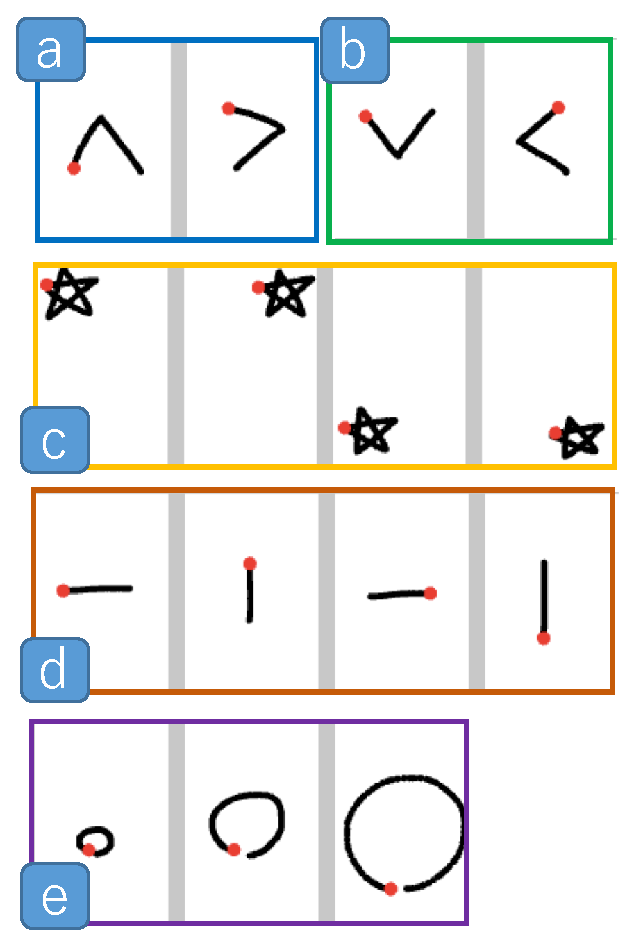
\includegraphics [width=0.5\columnwidth]{img/examples_V.eps}
\caption{ストロークの形状と書き順は同じであるが,大きさ (e), 向き (a) (b) (d), 位置 (c) が異なる,単一ストロークからなる手書きジェスチャの例}
\label{fig:examples_V}
\end{figure}


認識速度の観点でいえば,DTW~\cite{Tappert:1982:CSR:1664966.1664979, Salvador:2007:TAD:1367985.1367993}は,HCI分野において,手書きジェスチャ認識を実現するために広く採用されているアルゴリズムであり,単純にストロークを構成する点の距離を比較するのみであるため,こちらも,手書きジェスチャを構成するストロークの形状と書き順は同じであるが,大きさ,向き,位置に関して異なるストロークを識別することは可能である.しかしながら,単純なアルゴリズムによって認識率を向上させるために,非常に計算量が大きいといった問題点がある.

しかしながら,ユーザ調査により,これまでに述べたきたような,ストロークの形状と書き順は同じであるが,大きさや向きや位置が異なる単一ストロークからなる手書きジェスチャ~(図\ref{fig:examples_V})をアプリケーションユーザが入力として用いることを要望していることが導かれた.
これらは既に述べたように既存の\$-Family Recognizerにおいて識別できないため,これらのようなユーザ定義手書きジェスチャを入力として用いるようなアプリケーションを開発したい開発者は既存の\$-Family Recognizerを認識アルゴリズムとして用いることができない.また,これらを識別可能なRubine classfierやDTWなどを採用した場合は,認識率や認識速度において十分なパフォーマンスを得られない可能性がある.


\section{目的}
本研究の目的は,\$1を拡張し,単一ストロークからなる手書きジェスチャに対し,ストロークの大きさ,向き,位置に関して識別可能としながらも,\$1と比較し認識率の低下と認識速度の低下を最小限に抑えることを実現した\$-Family Recognizer開発することである.
我々はこの,ストロークの大きさ,向き,位置に関して``V''ariant~(不変)なストロークを認識する\$-Family Recognizerを\$Vと名付けた.
\$Vは\$1にアルゴリズムを少し追加するのみであるため,どのような開発環境においても実装可能であることも目標としている.
また,\$1と同様,少ない学習データにおいて高い認識率を示すことも目標としており,これは,アプリケーションユーザが手書きジェスチャを独自に定義することが可能であることを示している.
また,大きさ,向き,位置に関して識別可能な既存アルゴリズムと比較することによって,\$Vの有用性を示すことも本研究における目的とする.


%\$Vは,大きさ,向き,位置を特徴量として用いることによって,それらに依存するストロークを識別可能とした.
%その際,学習データを元に,ストロークを形状と書き順ごとに分類し,認識に用いる特徴量に重み付けをすることによって考慮すべき特徴量を適切に配分し,\$1と比べても遜色のない認識率と認識速度を実現した.
%\$1を改良した多くのアルゴリズムを用いず,\$1を拡張した理由は,\$1にて計算された,大きさ,向き,位置の特徴量を再利用することによって,\$1アルゴリズムと比べて,アルゴリズムの追加量を抑えること,認識速度の低下を抑えることにつながるからである.

\section{貢献}
本研究における手書きジェスチャ認識アルゴリズム\$Vの貢献を以下に示す.
\begin{itemize}
\item 手書きジェスチャを構成するストロークの形状と書き順は同じであるが,大きさ,向き,位置に関して異なる手書きジェスチャ識別することが可能なアルゴリズムを開発した.
\item 少ない学習データにおいて認識率を向上させるためのアルゴリズムを開発した.
\item 認識速度を向上させるためのアルゴリズムを開発した.
\item どのような開発環境においても実装可能な軽量なアルゴリズムを開発した.
\end{itemize}

\section{本論文の構成}
第1章では,研究背景と目的を述べた.第2章では,関連研究を述べる.第3章では,本研究の動機にもなった,アプリケーションユーザが入力として用いたい手書きジェスチャの調査について述べる.第 4 章では,\$Vの拡張元である\$1アルゴリズムについて述べ,第5章において,\$Vアルゴリズムの詳細について述べる.第6章では,\$Vのアルゴリズムとしての性能評価実験について述べる.第7章では,\$Vを用いたアプリケーション例を述べる.第8章では,\$Vアルゴリズムの今後の展望について議論する.第9章では,本研究の結論を述べる.
なお,付録 A に\$Vアルゴリズムの擬似コードを示す.
%付録 B に第 3章のユーザ調査に用いた調査同意書を,付録 B に調査について説明する際に用いた説明書を,付録 Dに第6章の評価実験に用いた実験同意書を示す.


%関連研究
\chapter{関連研究}
本章にて,本研究に関連する研究を述べる.本研究では,ユーザが定義する手書きジェスチャを高速に認識し,かつ容易に実装可能な軽量なアルゴリズムを開発している.また,本研究において開発したアルゴリズム\$Vはストロークの大きさ,向き,位置に関して識別可能な\$-Family Recognizerである.以上を踏まえ,本研究の関連研究を,一般的な手書きジェスチャ認識アルゴリズムの研究,ユーザ定義に特化した手書きジェスチャ認識アルゴリズムの研究,Progamming by Exampleに関する研究,\$-Family Recognizerに関する研究,手書きジェスチャ認識を可能にするツールキットに関する研究,手書きジェスチャの評価に関する研究に分類する.
本章にて,それらの研究について述べた後,最後に本研究における手書きジェスチャ認識アルゴリズムである\$Vの位置づけについて述べる.

\section{手書きジェスチャ認識アルゴリズム}
文字,ストロークの形状,手書きジェスチャなどの認識は,長く広く研究されている分野であり,多くのアルゴリズムにより実現されてきた.
finite state machines~\cite{Hong00constructingfinite}~(有限オートマトン)は,有限個の状態と遷移と動作の組み合わせからなる論理モデルであり,ある「状態」において,何らかのイベントや条件によって別の状態へ「遷移」することを繰り返すことによって最終的な認識結果を導く.高い認識精度を示すためには,より詳細なモデルの定義が必要となる.
Hidden Markov Models~(HMMs)~\cite{Anderson2004HiddenMM,Sezgin:2005:HES:1040830.1040899, Cao:2005:EOA:1089508.1089540}~(隠れマルコフモデル)は,観測された出力の系列から,内部の状態系列を統計的に推測するためのアルゴリズムである.
neural networks~\cite{Pittman:1991:RHT:108844.108914}は脳機能の特性を計算機上に応用したアルゴリズムであり,大量の学習によってモデルを最適化し,多次元量のデータで線形分離不可能な問題に対して小さい計算量で良好な解を得ることができる.
feature-based statistical classifiers~\cite{Cho:2006:NGR:1711617.1711649,Rubine:1991:SGE:127719.122753}は,大量の学習データによる特徴量をもとに学習データをクラスタリングし,より低次元な認識モデルを生成するためのアルゴリズムである.
ad hoc heuristic recognizers~\cite{Anthony:2010:LMR:1839214.1839258, Wilson:2003:XUI:642611.642706}は,「限定的な」認識アルゴリズムであるため,事前に定義されたジェスチャのみ認識することができる.すなわち,アプリケーション実行時において,新たな学習データを追加した場合に,新たなヒューリスティック関数を定義しなければならないため,アプリケーションユーザが独自にジェスチャを定義することができない.
template matching~\cite{Kara:2005:ITS:1652319.1652712, Kristensson:2004:SLV:1029632.1029640}は.主に画像処理に利用され,学習データと入力データの画像をそれぞれ走査し,画像上の各位置における類似度を算出するアルゴリズムであり,手書き文字にも応用されている.

これらアルゴリズムはオンライン文字認識及びオフライン文字認識双方においてしばしば用いられるアリゴリズムである.オンライン文字認識とは,タブレットなどにペンや指などによって入力された文字を認識する技術の総称であり,オフライン文字認識とは,紙に書かれた文書イメージを光学スキャンし,そのイメージを自動的にコンピュータで処理可能なテキストデータに変換する技術の総称である.しかしながら,これらアルゴリズムは,高い認識精度を示す認識モデルを生成するために膨大な数の学習データが必要であり,素早く手書きジェスチャ入力のテストしたい場合において不向きであるだけでなく,アプリケーションユーザが独自にジェスチャを定義する上で実用的であるとは言えない.また,これらアルゴリズムを実装することは,それぞれの分野に精通していない開発者にとって困難である.

\section{ユーザ定義に特化した手書きジェスチャ認識アルゴリズム}
ユーザ定義の手書きジェスチャを認識できるアルゴリズムのうち,少ない学習データによって高い認識率を示すアルゴリズムを示す.
Rubine classifier~\cite{Rubine:1991:SGE:122718.122753}及びDynamic programming~(DTW)~\cite{Tappert:1982:CSR:1664966.1664979}などは,少ない学習データにおいてジェスチャ認識可能なアルゴリズムであるが,Rubine classifierは認識率が高いとは言えない.また,13もの特徴量を適切に選ばないと,認識率が低下するという欠点があり,それぞれの特徴量が認識結果に及ぼす影響について深い知識がない場合,特徴量の選定が難しい.このように認識に用いる特徴量を単に増やすことは,それについて識別できることにつながるが,ロバスト性の低下を招くという欠点もある.DTWはアルゴリズムが簡潔であるが,計算量が非常に大きいという問題点がある.計算量を改善したFast DTW~\cite{Salvador:2007:TAD:1367985.1367993}が開発されたが,アルゴリズムは複雑になっており,プロトタイピング環境開発向けとは言い難い.

\section{Programming by Example}
Programming by Exampleとは,学習データをもとに,認識モデルを自動生成する手法である.
システムに明示的に学習データを例として与え,ユーザの意図や好みを推論することにより,ユーザの意図に沿った処理を行ったり,処理自体を削減したりすることが可能となる~\cite{110003743975}.この手法は手書きジェスチャ認識においても活用されている.
例えば,Tarantaら~\cite{Taranta:2016:RPA:2984511.2984525}は,Gesture Path Stochastic Resampling~(GPSR)という,学習データをもとに人間が書くような手書きジェスチャを生成するためのアルゴリズムを考案した.このように,あるデータをもとにそのデータにより近く,より自然な新たなデータを自動生成するアルゴリズムとして,Syntetic Data Generation~(SDG)~\cite{conf/iccv/NavaratnamFC07,Shotton:2011:RHP:2191740.2192047,Galbally_syntheticgeneration,Lundin:2002:SFD:646280.687684,Gatos:2005:SAK:1106779.1106876,Rodriguez-Serrano:2012:SQH:2240326.2240755,Fischer:2013:GLS:2501115.2501123}があり,これらのアルゴリズムは手書きジェスチャを始めとするパターン認識において,学習データをもとにユーザの意図に沿った認識モデルを自動生成するために用いられている.また,Perlin noise~\cite{Perlin:1985:IS:325165.325247}あるいは,SigmaLognormal~\cite{SigmaLognormal}も,手書きジェスチャを自動生成するためのアルゴリズムとして広く利用されている.GPSRはユーザから得られたそれぞれの手書きジェスチャの特徴をもとに,そのジェスチャの認識率が高くなるような自動生成方法を計算することによって,Perlin noiseあるいは,SigmaLognormalを用いた場合よりも高い認識率を示した.これらは,学習データを大量に自動生成することができるため,少ない学習データにおいて高い認識率を示す,ユーザ定義に特化した手書きジェスチャ認識アルゴリズムでもある.

\section{\$-Family Recognizer}
\$1~\cite{Wobbrock:2007:GWL:1294211.1294238}は,\$-Family Recognizerの先駆的なアルゴリズムであり,\$1を改良したアルゴリズムは,\$-Family Recognizerと呼ばれている.
\$1は,少ない学習データにより,高い認識率を示すアルゴリズムであるため,ユーザが独自にジェスチャを定義するジェスチャ認識システムを開発することが可能である.また,開発者は,自身のシステムに,簡単な数式のみを含む,およそ100行からなるアルゴリズムを追加するのみによって,単一ストロークからなるジェスチャ認識を行うことが可能であるため,手書きジェスチャ認識をプロトタイピングするような環境において実装可能である.\$1は入力データと学習データの対応する点のユークリッド距離が最小となるような最適な角度を探索することによってジェスチャ認識を行っている.
しかしながら,ストロークを,大きさ,向き,位置に不変にしているため,それらの特徴量が異なるようなジェスチャを認識することができない.したがって,そのようなジェスチャを認識するようなアプリケーションを開発したい開発者は\$1を自身のシステムに採用することができない.

\$1が認識することができないジェスチャを認識するために,これまで\$1を拡張した\$-Family Recognizerが開発されてきた.

\$N~\cite{Anthony:2010:LMR:1839214.1839258}は,複数のストロークからなるジェスチャを認識することを可能にし,識別可能なストロークを大幅に増やすことに成功した.\$Nは,ストロークを複数の単一ストロークに分割し,それぞれの単一ストロークを\$1の手法によって認識した.また,考えられる複数の単一ストロークの組み合わせを自動的に計算することによって,ストロークの向きや書く順番にロバストな認識も可能にした.

Quick\$~\cite{Reaver:2011:MQU:2021164.2021183}は,\$1の改良であり,最短距離法によるクラスタリングによって,対応する点のユークリッド距離が最小となる入力データと学習データの組み合わせを効率的に探索し,認識速度を高速化するアルゴリズムである.

Protractor~\cite{Li:2010:PFA:1753326.1753654}も\$1に対し,認識速度の面において改良したアルゴリズムである.最適な角度を探索する際に,Golden Section Search~(GSS)~\cite{Press:1992:NRC:148286}%(pp. 397-402)
を用いた\$1とは異なり,閉形式解を用いることによって,より高速に探索することを可能とした.

\$N-Protractor~\cite{Anthony:2012:NFA:2305276.2305296}は,\$Nに対し,Protractorの手法を用いることによって,より高速にかつ,より正確に複数のストロークからなるジェスチャを認識することを可能にした.

1 cent Recognizer~\cite{Herold:2012:CRF:2331067.2331074}は,\$1よりも高速であり,アルゴリズムも非常に単純であるため実装が容易であるが,認識可能なジェスチャの種類や,認識率の観点からみると実用的であるとは言えない.

\$P~\cite{Vatavu:2012:GPC:2388676.2388732}は,ストロークを構成する点をPoint Cloudとして扱うことによって,\$N-Protractorよりも,メモリ消費量や認識速度の点において効率的なアルゴリズムである.

Penny Pincher~\cite{Taranta:2015:PPB:2788890.2788925}は,ストロークを構成する点間のベクトルを用いることによって,これまでの\$-Family Recognizerと比べて,より高速にかつ,正確に認識することを可能にした.

これらの\$-Family Recognizerは,2次元のストロークからなる手書きジェスチャを認識をすることが可能であり,\$1に対し,アルゴリズムを簡略化したり,認識速度を高速化したり,認識率を高くしたり,認識できるストロークの種類を増やしたりするなどして,繰り返し改善されてきた.

しかしながらこれらのアルゴリズムは,ストロークの特徴量である,大きさ,向き,位置に関して,そのいずれかあるいはすべてについて不変になるようなアルゴリズムを採用することにより,それらの特徴量についてロバストなジェスチャ認識を実現し,その結果認識率や,認識速度の向上を実現してきた.
それらを不変にしないことは,その特徴量について識別できるようになることにつながるが,不変にしない特徴量についてはロバストではなくなるため,認識率の低下や認識速度の低下を招く恐れがある.例えば,1 cent Recognizerはストロークを構成するすべての点の中心座標から,それぞれの点へのユークリッド距離のみを特徴量とし,入力データと学習データの特徴量の差が最小となるストロークを探索しているため,ストロークの形状と書き順は同じであるが,大きさ,向き,位置に関して異なるストロークを識別することは可能である.しかし,それぞれの特徴量についてロバストでないため,それぞれの特徴量についてわずかでさえ異なる場合,認識できないことが多々あり,結果的に認識率の低下を招いている.
%認識速度の観点でいえば,DTWは,単純にストロークを構成する点の距離を比較するのみであるため,こちらも,ストロークの形状は同じであるが,大きさ,向き,位置に関して異なるストロークを識別することは可能であるが,認識率を向上させるために,非常に計算量が大きい.

\section{手書きジェスチャ認識を可能にするツールキット}
%プロトタイピング環境向けに開発できるように,
手書きジェスチャ認識を簡単に開発することが可能なツールキットも開発された~\cite{Henry:1990:IGS:97924.97938,Landay:1993:EEU:259964.260123,Myers:1997:AEN:262050.260628}.SATIN~\cite{Hong:2000:STI:354401.354412}はジェスチャ認識の開発を容易にするだけでなく,ペンベースのユーザインタフェースを採用し,ジェスチャ認識のモデルを手書きによって定義することができるツールキットである.
%Henryら~\cite{Henry:1990:IGS:97924.97938},LandayとMyers~\cite{Landay:1993:EEU:259964.260123},及びAmulet toolit~\cite{Myers:1997:AEN:262050.260628}は,手書きジェスチャを入力として用いたアプリケーションを開発するためのツールキットである.
これらは,開発を手助けするのに非常に強力であるが,対応可能な開発環境が限定されているため,自身の環境に適用できない場合がある.

\section{手書きジェスチャの評価研究}
手書きジェスチャは,これまで様々な研究において入力手法として用いられており,曲線などを用いた複雑な構造からなる手書きジェスチャ~\cite{Lu:2011:GAT:1978942.1978972,Li:2010:GST:1866029.1866044,Moran:1997:PIT:263407.263508,Hinckley:2007:ISS:1240624.1240666,Appert:2009:USC:1518701.1519052,Liao:2008:PGC:1314683.1314686,Zeleznik:2008:LCD:1449715.1449741}や,
1本あるいは2本の直線のみからなる単純な構造からなる手書きジェスチャ~\cite{Kurtenbach:1993:LEP:164632.164977}などが用いられている.
Bragdonら~\cite{Bragdon:2011:EAT:1978942.1979000}は,これらの研究において用いられる手書きジェスチャのうち,利用頻度の高い手書きジェスチャを抜粋し,それらをスマートフォンやスマートウォッチに対して入力する際に,どのような場面においてどのような手書きジェスチャが求められているのかを評価した.
Bragdonらは,アイズフリーによる操作及び歩行時における片手操作のみならず,立ち止まって端末を見ながら操作する場面でさえも,曲線などを用いた複雑な構造からなる手書きジェスチャよりも,1本あるいは2本の直線からなる単純な構造からなる手書きジェスチャの方が,認識率が高く,入力するまでの速度が速いため,ユーザによる利用頻度が高いということを示した.

\section{本研究の位置づけ}
本研究における手書きジェスチャ認識アルゴリズム\$Vは,アルゴリズムが簡潔である\$1に,簡単な数式からなるアルゴリズムを追加するのみによって実装できるため,パターン認識に関する深い知識がなくとも実装可能である上,どのような開発環境においても実装可能である.また,少ない学習データにより高い認識率を示すため,ユーザ定義手書きジェスチャを認識することが可能であり,既存のユーザ定義に特化した手書きジェスチャ認識アルゴリズムと比較し,認識率及び認識速度において高い性能を示すアルゴリズムである.

\$Vは,既存の\$-Family Recognizerとは違い,ジェスチャの形状と書き順が同じであるが,大きさ,向き,位置に関して異なる手書きジェスチャを識別することが可能である上,認識率及び認識速度において性能の低下を抑えたアルゴリズムである.また,\$Vは,得られた学習データから,ユーザがそれぞれの手書きジェスチャをどのように区別して登録しているのかを推測するProgramming by Exampleの考え方に基づき,大きさ,向き,位置に関して異なる手書きジェスチャを識別するために必要な特徴量に高い重み付けをするという処理を施している.これにより,ロバスト性が維持され,結果的に認識率の低下を抑えている.また,識別するために必要なジェスチャのみに対し,類似度計算を行うことによって,認識速度の低下を抑えている.

これらに加え,\$Vは大きさ,向き,位置に関して異なる手書きジェスチャを識別することが可能であるため,ユーザは,曲線などを用いた複雑な構造からなる手書きジェスチャを多く考える必要がなく,1本あるいは2本の直線のみからなる単純な構造からなる手書きジェスチャを用いて,大きさ,向き,位置に関して様々なバリエーションを持たせた手書きジェスチャを考えるだけで良いといった利点がある.







%被験者への手書きジェスチャの調査
\chapter{ユーザ調査}
本章においては,本研究の動機にもなった,アプリケーションユーザが入力として用いたい手書きジェスチャの調査内容とその結果について述べる.

\section{アプリケーションユーザへの手書きジェスチャの調査}
単一ストロークからなる手書きジェスチャ認識を用いたシステムが,これまでにも多く開発されてきた.その中で,\$1は,  ~\cite{Hong:2000:STI:354401.354412, Landay:1993:EEU:259964.260123, Lin:2000:DFT:332040.332486}において用いられているような,一般的にスマートフォンやタブレット端末などのタッチパネルへの手書き入力やペン入力において良く用いられる,単一ストロークからなるジェスチャを抜粋し~(図\ref{fig:stroke_1}),それらについて認識率を計測した.\TODO{それぞれについて詳しく書く.}
しかしながら,ユーザ定義ジェスチャを用いた研究~\cite{Vatavu:2012:UGF:2325616.2325626, Bragdon:2011:EAT:1978942.1979000, Wobbrock:2009:UGS:1518701.1518866, Shimon:2015:EUB:2785830.2785890}の中には,単一ストロークからなるジェスチャであり,かつ,ストロークの形状は同じであるが,ストロークの向きや位置の違いを利用したジェスチャを入力に用いる場合があった.

そこで,普段スマートフォンを利用する場面,およびスマートフォンを入力デバイスとしPCを操作する場面を想定した時,どのようなアプリケーションに対し,どのような手書きジェスチャを入力として用いたいかを事前調査した.

\begin{figure}[!h]
\centering
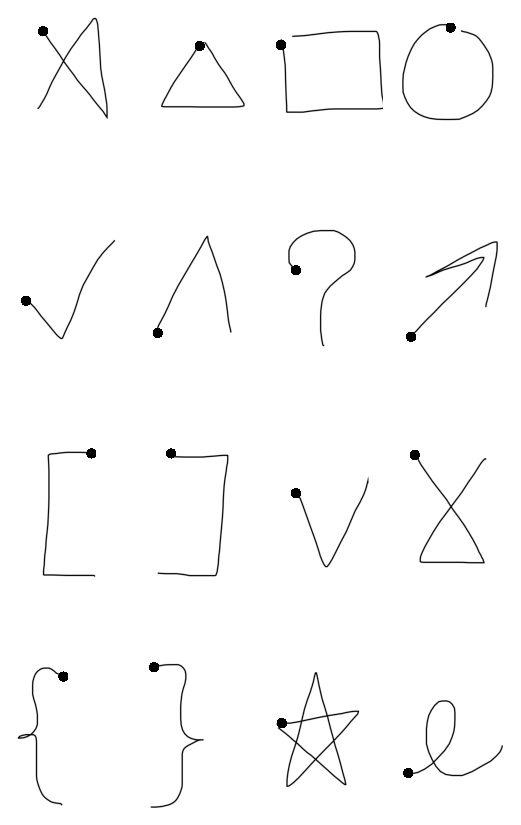
\includegraphics[width=0.4\columnwidth]{img/stroke_1.eps}
\caption{\$1において用いられる,一般的にスマートフォンやタブレット端末などのタッチパネルへの手書き入力やペン入力において良く用いられる,単一ストロークからなる手書きジェスチャの例}
\label{fig:stroke_1}
\end{figure}

\section{被験者}
被験者は普段からスマートフォンを使用している大学院生の男性6名である.年齢は21〜27歳~(平均23.8歳)であり,全員右利きであった.6名の被験者の中にはコンピュータサイエンスあるいはユーザインタフェースを専攻している人が4名存在し,残りの2名は,社会工学を専攻している男性と,エンジニアとして働いている男性であった.被験者は全員日頃からスマートフォンを使用していた.

%\section{調査に用いた機器}
%実験には,入力端末であるスマートフォンとしてiPhone5を用い,実験における入力領域は1.94'' × 3.18''であり,解像度は640 × 1036である~(図\ref{{fig:screenshot}}).

 %\begin{figure}[!h]
%\centering
%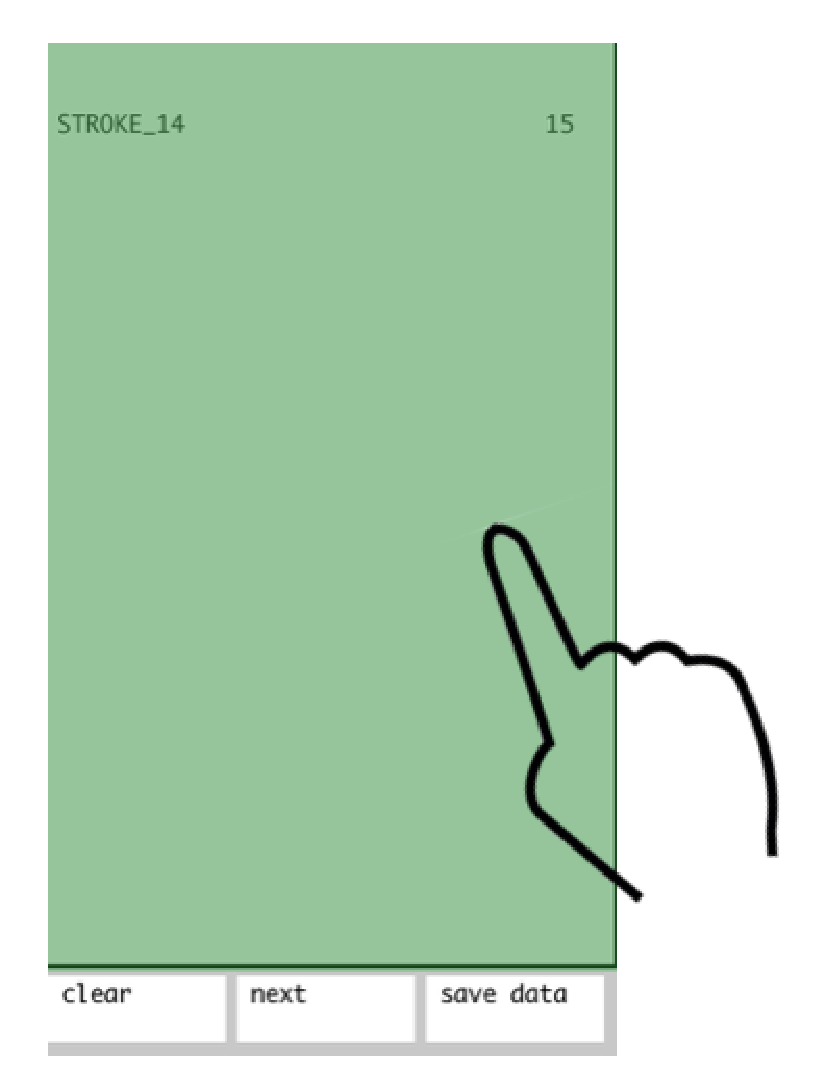
\includegraphics[width=0.4\columnwidth]{img/screenshot.eps}
%\caption{The screen shot on the smartphone. The green area is the input area}
%\label{fig:screenshot}
%\end{figure}

\section{調査手順}
%教示を詳しく書く
%使いたいジェスチャを入力することを示す
我々はまず,被験者に調査の目的を説明した.
その後,普段スマートフォンを利用する場面,およびスマートフォンを入力デバイスとしPCを操作する場面を想定した時,どのようなアプリケーションに対し,どのような手書きジェスチャを入力として用いたいかを20以上考えるよう指示し,自身のスマートフォンに対し実際に入力しながら考えるよう指示した.
%図\ref{fig:screenshot}における緑色の領域部分にジェスチャを入力するよう指示した.
その際,ジェスチャを入力する姿勢は次の3つの姿勢~(姿勢1,姿勢2,姿勢3)から,実際に自分がそのジェスチャを入力として用いるときに入力する姿勢として1つ選んでもらった.
\begin{enumerate}
\item 机にスマートフォンをおいて,利き手の人差し指によって入力する.
\item 利き手でスマートフォンを握りながら,同じ利き手の親指によって入力する.
\item 利き手とは反対の手でスマートフォンを握りながら,利き手の人差し指によって入力する.
\end{enumerate}
被験者は,全ての姿勢を座って入力するよう指示された.
また,入力ジェスチャとして,単一ストロークからなるよう指示した.

入力として用いたい手書きジェスチャを1つ考えるたびに,我々は付録\TODO{何の付録か}に示す紙にそのジェスチャをボールペンによって書くよう指示した.またそれに加え,そのジェスチャを入力した姿勢~(1〜3),そのジェスチャをどのアプリケーションに対して用いたいのかも同時に書くよう指示した.


\section{調査結果}
図\ref{fig:elicetated_strokes}は,6人の被験者から得られた手書きジェスチャ一覧である.

図\ref{fig:elicetated_strokes}において,例えば音楽再生アプリケーションにおいて,早送り,巻き戻し,音量の上げ下げ,といったような前後への移動や,値の上げ下げなど,対になるような操作に対して,向きや大きさの違いを用いて入力する要望があった.また,ブラウザアプリケーションにおいて,位置によって登録先のブックマークを変える,ページ内における表示位置をジェスチャの入力位置に対応させる,といったように,位置の違いを操作対象先の違いに割り当てたり,現在操作しているものの位置に対応付けるといった要望があることがわかった.

また,片手で操作する場面~(姿勢2)においては,難しいストローク操作ができないため,極力簡単なストロークを用い,かつ,大きさ,向き,位置の特徴量を利用して入力する要望があることも分かった.
\TODO{ここら辺もうちょい詳しく書く?}

\begin{figure*} [t]
 \begin{center}
  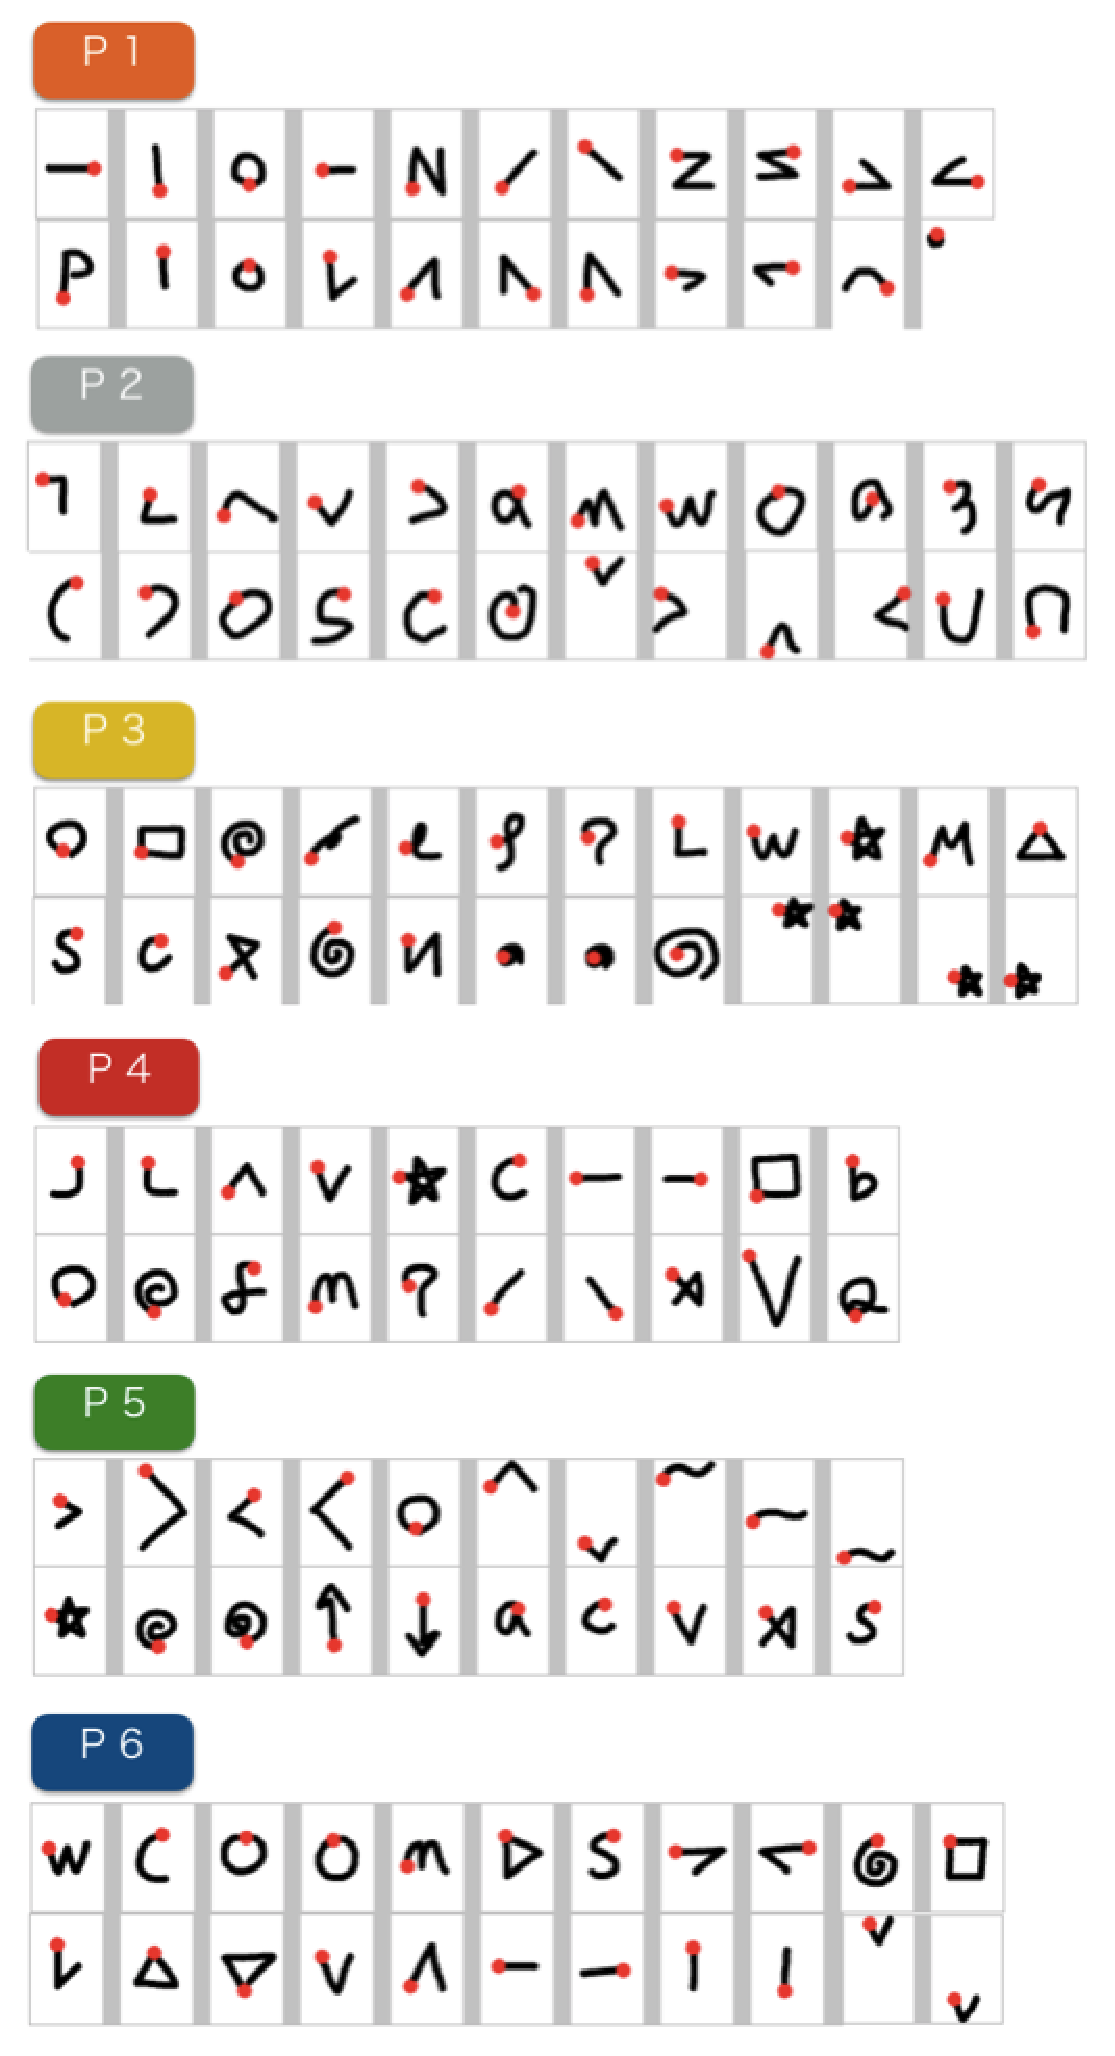
\includegraphics [width=0.7\columnwidth]{img/elicetated_strokes.eps}
  \caption{調査において6人の被験者~(P1〜P6)から得られた,用いたい手書きジェスチャの一覧}
  \label{fig:elicetated_strokes}
 \end{center}
\end{figure*}

\$Vは,図\ref{fig:elicetated_strokes}が示すような,ジェスチャの形状や書き順は同じでも,大きさ,向き,位置に関して異なる手書きジェスチャを認識することが可能なアルゴリズムであり,今回調査を行った被験者の要望を満たすことのできる手書きジェスチャ認識である.


%\$Vは,\$1にアルゴリズムを少し追加するだけで,\$1が示す認識率と認識速度を維持しつつ,図が示すような,ジェスチャの形状は同じでも,大きさ,向き,位置に関して異なるジェスチャ認識アルゴリズムである.






%$1
\chapter{\$1アルゴリズム}
\$Vは\$1の拡張である.そこで本章にて,\$1アルゴリズムを述べる.

\section{特徴}
ユーザが入力した手書きジェスチャは,図\ref{fig:strokes}のように複数の点によって構成され,すでに登録された手書きジェスチャと,それぞれの点を比較することによって,どの手書きジェスチャと一致しているかが判別される.しかしながら,これらの手書きジェスチャを構成する複数の点は,入力に用いられるハードウェアやソフトウェアに依存した速度によってサンプリングされる.それらに加え,人間によって入力される手書きジェスチャにはばらつきがあるため,入力される手書きジェスチャを構成する点の数は入力されるたびに異なる.
そのため,ユーザが入力した手書きジェスチャと,すでに登録された手書きジェスチャを比較するにあたり,手書きジェスチャを構成する点どうしを単純に比較することは困難であるといえる.


例えば,図\ref{fig:strokes}の手書きジェスチャは,入力速度によって手書きジェスチャを構成する点の数が異なる例である.それだけでなく,ジェスチャ自体の大きさや向きも異なる.これらは,手書きジェスチャ認識においてジェスチャを比較する上で,1つのハードルとなっている.
これらのような手書きジェスチャによって生じる問題点に対処しつつ,高い認識率を示し,かつどのような開発環境においても実装可能な簡易的なアルゴリズムを実現するために,\$1は以下のような基準に従うようなアルゴリズムの実現を目指した.

\begin{itemize}
\item ハードウェアやソフトウェアのセンシング及び入力する速度などによって変わるサンプリングされる点の数の違いに対してロバストであること.
\item 手書きジェスチャの大きさ,向き,位置に不変な認識をすること.
\item 数学的な高度な知識やテクニックをを必要としないこと(例えば,逆行列,微分,積分など)
\item 少ないコードによって実装できること.
\item 認識速度が速いこと.
\item ソフトウェア開発者やアプリケーションユーザが,独自に手書きジェスチャを定義できること.
\item N-best listに関して,高い識別能力を示すスコアを示すこと.
\item 図\ref{fig:stroke_1}のような単一ストロークからなる手書きジェスチャを認識するにあたり,HCI分野において多く用いられる既存の複雑な手書きジェスチャ認識アルゴリズムと比べても,高い認識率を示すこと.
\end{itemize}

ここで,N-best listとは,N個の学習データそれぞれに対する入力データとの類似度を降順に並べたものであり,N-best listの1番目と2番目のスコアの差が大きいほど,高い識別能力を示しているといえる.

次に,これらの基準に従うように開発された\$1のアルゴリズムを述べる.
アルゴリズムは大きく4つのステップから構成される.


\section{\$1アルゴリズムの4つのステップ}
4.1節において述べた基準を満たすために,入力データ及び学習データは4つのステップを経た後に比較される.
4つのステップは,リサンプル,向きと大きさの正規化,位置の正規化,類似度を高くするための最適な角度の選定からなる.

\subsection{リサンプル}
前節において述べたように,手書きジェスチャを構成する点の数は,ハードウェアやソフトウェアのセンシング及び入力する速度などによって変わる.特に,入力速度の違いによる点の数の違いは顕著である(図\ref{fig:strokes}).

\begin{figure} [!h]
\centering
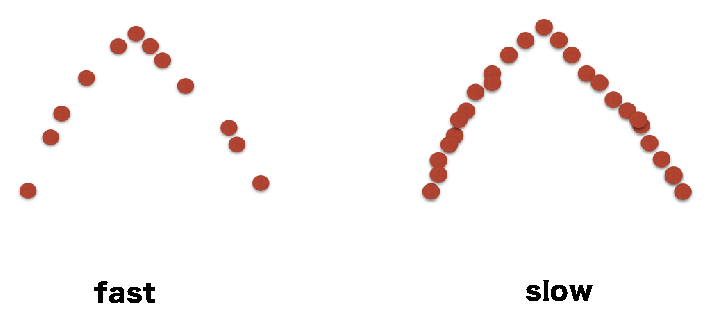
\includegraphics [width=0.6\columnwidth]{img/strokes.eps}
\caption{複数の点から構成されるストローク.同じストロークでも,入力される速度によって点の数が異なる.}
\label{fig:strokes}
\end{figure}

点の数が違うことにより,入力データと学習データの手書きジェスチャを構成する点を互いに比較することが困難となっている.そこで,図\ref{fig:resample}に示すようにN個の等間隔に並ぶ点にリサンプルする.N個の点にリサンプルすることは,生のデータを扱うことと比べて正確なデータを扱っているとはいえず認識精度が落ちる可能性があるが,入力データと学習データ双方の手書きジェスチャの点の数が等しくなるため,容易に互いの対応する点を比較できる.

\begin{figure} [!h]
\centering
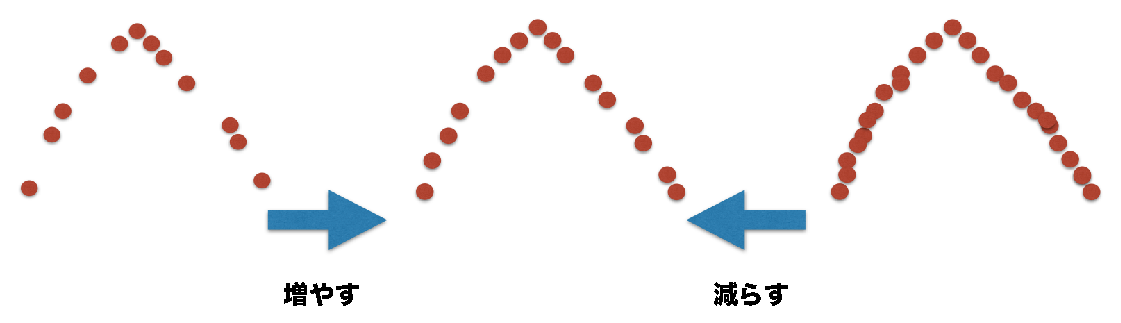
\includegraphics [width=0.8\columnwidth]{img/resample.eps}
\caption{リサンプリングの例.点の数が異なる同じジェスチャも,同じ数の点へとリサンプリングされる.}
\label{fig:resample}
\end{figure}

リサンプルすることは,既存の手書きジェスチャ認識アルゴリズムにおいても用いられている~\cite{Plamondon:2000:OOH:331097.331275, Tappert:1990:SAO:83123.83137, Kristensson:2004:SLV:1029632.1029640, Zhai:2003:SWS:642611.642630, Tappert:1982:CSR:1664966.1664979}.
%\$1はこれらのアルゴリズムを採用するとともに,これらのアルゴリズムとは違い向きに不変なアルゴリズムを提供する.また,
%手書きジェスチャを構成する点の数をリサンプルすることなく実行可能なDTWと比較している.

%N個の等間隔に並ぶ点にリサンプルする方法を図に示す.
%\TODO{リサンプルの仕方を図で説明}

また,リサンプルされる点の数Nは,32$\leq$N$\leq$256の場合,N$=$64の場合に認識率,認識速度双方において高いパフォーマンスが得られることも\$1において報告されている.

\subsection{向きと大きさの正規化}
リサンプルされた手書きジェスチャの向きを``indicative angle''として定義する.indicative angleとは図\ref{fig:orientation}のように,手書きジェスチャの書き始めの一番最初の点の座標,手書きジェスチャを構成する点全てによる中心座標,0度方向によって形成される角度である.そして,indicative angleに沿って,全てのジェスチャを回転させる.これにより,ジェスチャは向きが正規化される.

\begin{figure} [!h]
\centering
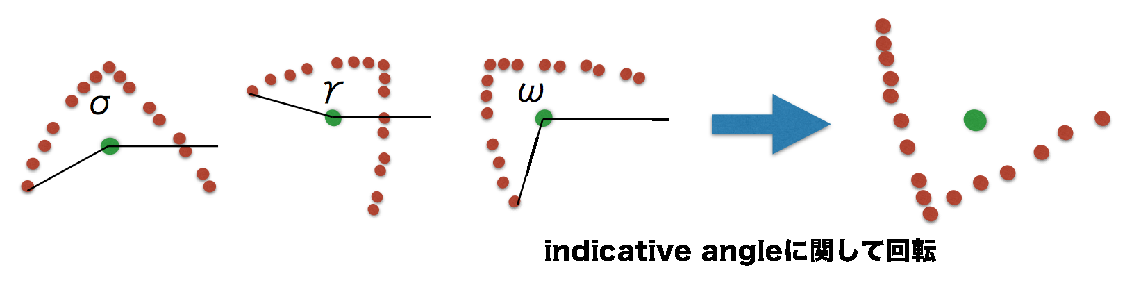
\includegraphics [width=0.8\columnwidth]{img/orientation.eps}
\caption{向きに正規化する例.向きが異なったとしても,同じ向きになるように回転する.}
\label{fig:orientation}
\end{figure}

向きによって正規化されたジェスチャの大きさを``boundingbox''として定義する.boundingboxとは図\ref{fig:size}のように,ジェスチャに隣接するような矩形である.全てのジェスチャについて,boundingboxをある一定の大きさの矩形に正規化することによって,ジェスチャは大きさが正規化される.

\begin{figure} [!h]
\centering
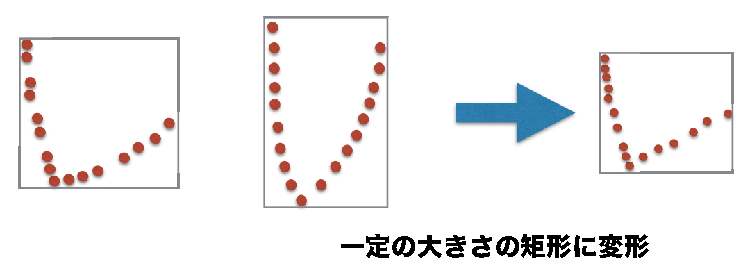
\includegraphics [width=0.7\columnwidth]{img/size.eps}
\caption{大きさに正規化する例.大きさが異なったとしても,同じ大きさになるように変形する.}
\label{fig:size}
\end{figure}

\subsection{位置の正規化}
向きと大きさによって正規化されたジェスチャの位置をジェスチャを構成する全ての点による中心座標として定義する(図\ref{fig:position}における緑色の点).全てのジェスチャについてこの中心座標を(0, 0)へと移動させることによって,位置が正規化される.

\begin{figure} [!h]
\centering
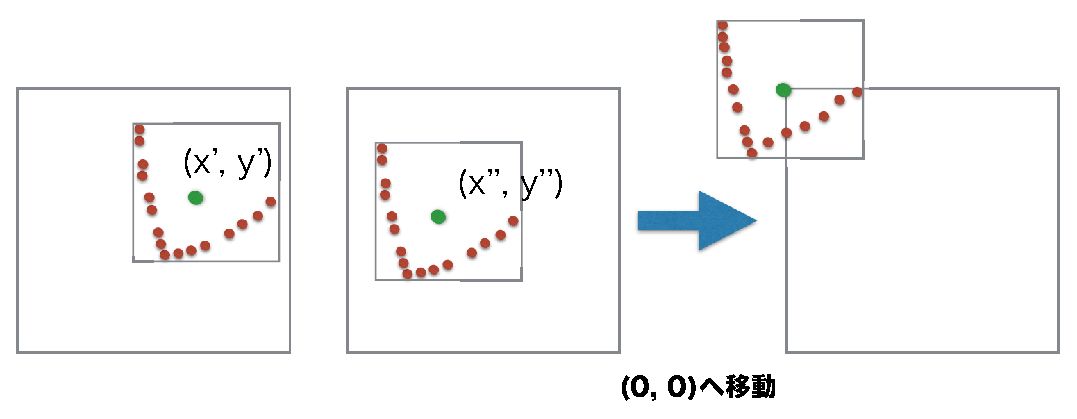
\includegraphics [width=0.8\columnwidth]{img/position.eps}
\caption{位置に正規化する例.位置が異なったとしても,同じ位置になるように移動する.}
\label{fig:position}
\end{figure}

\subsection{類似度を高くするための最適な角度の選定}
リサンプルされた2つの手書きジェスチャ構成する点について,1つずつ対応する点どうし比較するにあたり,$1^\circ$ずつ手書きジェスチャを回転させながら,最も類似度が高くなるような角度を見つけた上で,類似度を算出する方法~\cite{Kara:2005:ITS:1652319.1652712}がある.しかしながらこの方法は認識のために膨大な時間を要することになる.全ての学習データの数が30程度の場合そのような方法でも十分な速度によって認識することが可能であるが,\$1は黄金分割探索~\cite{Press:1992:NRC:148286}を用いることによって最も類似度が高くなるような角度を求める.
黄金分割探索とは,単峰関数(極値が1つしかない関数)において,極値を求めるための方法(局所探索法)のうち効率的な方法の1つであり,極値が存在することが自明な範囲において極値を逐次的に求める方法である.

例えば図\ref{fig:golden}において,$f(x)$の関数があり,極小値$f(x')$を求める時に,$x1$と$x3$の間に極値が存在することが自明な時に,その範囲内に存在する$f(x2)$を求める.この時$x2$は$(x2 - x1) : (x3 - x2)$が黄金比~(1 : $\frac{1+\sqrt{5}}{2}$)となるように設定する.これが黄金分割探索といわれる所以であり,常に3点(この場合$x1$, $x2$, $x3$)が存在する.その後広い区間(この場合$x2$と$x3$の間)において,同様に黄金比によって分割し新たな$f(x4)$を得る.この時,$f(x4a)$ならば,極小値は$x1$と$x4$の間に存在するため,新たな3点は$x1$, $x2$, $x4$となる.$f(x4b)$ならば,極小値は$x2$と$x3$の間に存在するため,新たな3点は$x2$, $x4$, $x3$となる.このように,極小値が存在する範囲を徐々に狭めていくことによって,効率よく極値を求めることができる.

\begin{figure} [!h]
\centering
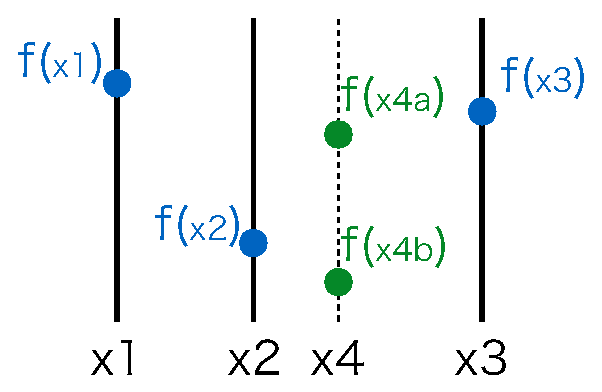
\includegraphics [width=0.4\columnwidth]{img/golden.eps}
\caption{黄金分割探索によって,極値を求める例.}
\label{fig:golden}
\end{figure}

\$1の場合,480個の手書きジェスチャにおいて,$\pm45^\circ$の範囲において極小値が存在することが発見され,極小値が存在する範囲が$2^\circ$になるまで黄金分割探索を行う.この時,入力データに類似する学習データが存在する場合あるいは存在しない場合においても,10ステップ後には極小値が求められることが発見された.

局所探索法の1つである山登り法~\cite{Park:2009:SFA:1464526.1465112,Department94prototypeand}を黄金分割探索の代わりに用いる場合,480個の手書きジェスチャにおいて,類似するジェスチャの場合およそ7.2ステップ後に極小値を求めることができるが,類似しないジェスチャの場合はおよそ53.5ステップ後に極小値が求められることが発見された.つまり学習データが10ずつ存在する$16種類の手書きジェスチャ=160$個のジェスチャにおいて,黄金分割探索は$160\times10=1600$ステップ必要であるのに対し,山登り法は$7.2\times10 + 53.5\times150=8097$ステップ必要であり,およそ80.2\%もの計算量の節約となっている.

このように,類似度を高くするための最適な角度を黄金分割探索によって効率的に求めることによって,認識速度の向上を実現している.

以上の4ステップをまとめ,入力データと学習データそれぞれを比較するまでの過程を図\ref{fig:onedoller_flow}に示す.
\begin{figure} [!h]
\centering
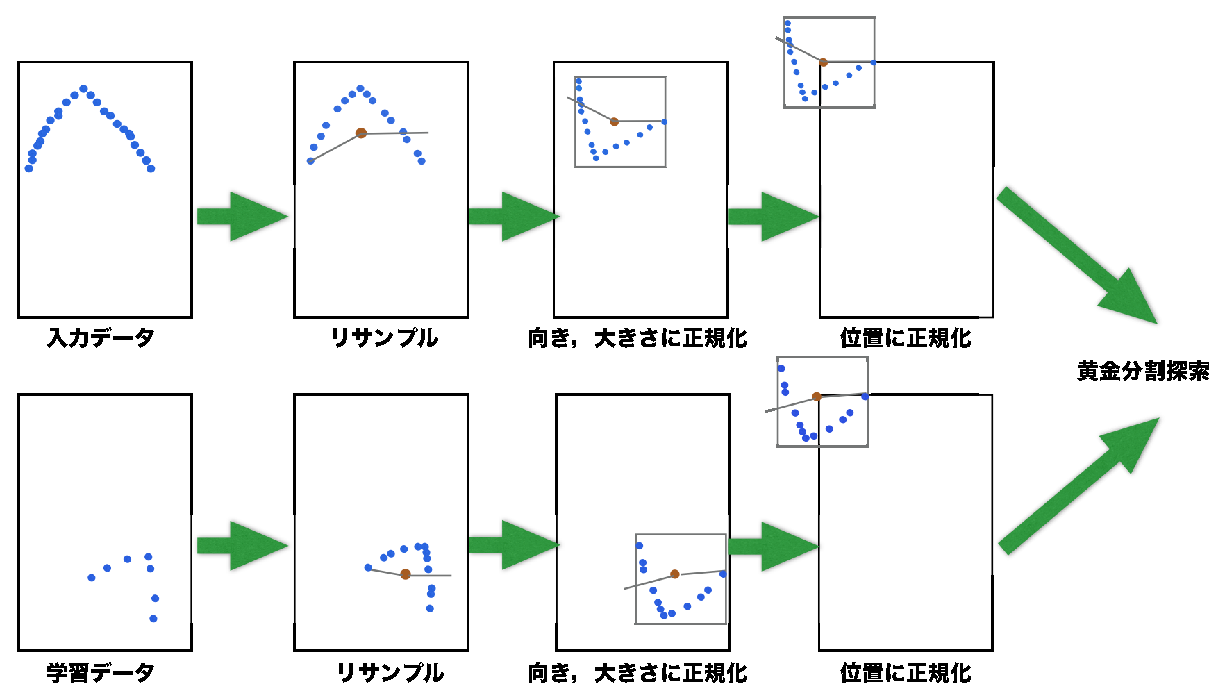
\includegraphics [width=0.9\columnwidth]{img/onedoller_flow.eps}
\caption{\$1アルゴリズムにおいて4つのステップを経て,入力データと学習データが比較されるまでの流れ.}
\label{fig:onedoller_flow}
\end{figure}

\section{類似度計算}
前節までの4ステップによって得られた入力データと学習データの最終的な類似度は式(4.1)によって表される.
\begin{equation}
score = 1 - \frac{d}{\frac{1}{2}\sqrt{size^2 + size^2}}
\end{equation}
ここで,$d$は対応する点どうしのユークリッド距離の全ての点に関する平均値であり,$size$は大きさに正規化するに用いられる矩形(正方形)の1辺の長さである.

\section{制約}
\$1は,手書きジェスチャを,大きさ,向き,位置に正規化することによってアルゴリズム全体を簡潔化したり,それぞれについてロバストな認識を可能にし認識率の向上を実現した.しかしながら,このことが原因により,幾つかの制約が存在する.

\begin{itemize}
\item 手書きジェスチャを大きさ,向き,位置によって識別しない.
\item 直線のような1次元の手書きジェスチャを認識することができない.
%\item 手書きジェスチャを入力する速度による識別ができない.
\end{itemize}


「手書きジェスチャを大きさ,向き,位置によって識別しない」ことに関しては,それぞれについて正規化しないようにアルゴリズムを変えることによって識別することが可能となる.しかしながら,正規化しないことにより,正規化しないものに関してはロバスト性が低下するため,結果的に認識率の低下を招く恐れがある.

「直線のような1次元の手書きジェスチャを認識することができない」ことに関しては,向き,大きさに関して正規化した際に図\ref{fig:line}のように,ストロークを構成する各点が分散してしまうためである.

\begin{figure} [!h]
\centering
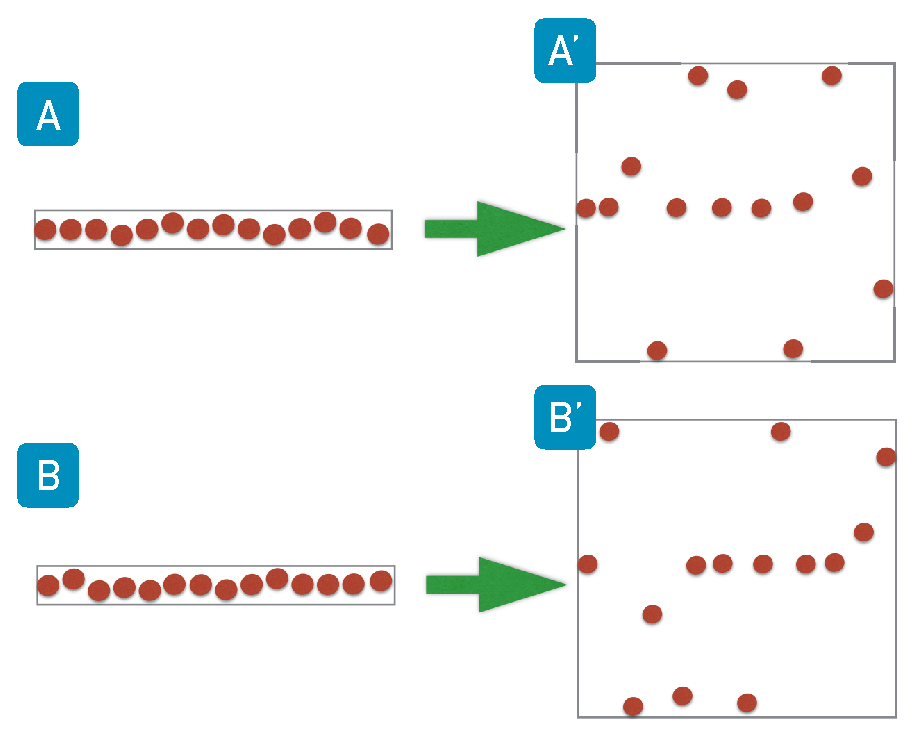
\includegraphics [width=0.6\columnwidth]{img/line.eps}
\caption{\$1が1次元の手書きジェスチャを認識できない理由.向き及び大きさに正規化することによって,ストロークを構成する各点は分散しまう.分散する前(A)及び(B)は類似しているが,正規化により分散した後(A')及び(B')は類似していないため,同じ手書きジェスチャとして認識されない.}
\label{fig:line}
\end{figure}

\$Vは,これらの問題点を解決したアルゴリズムである.

%「手書きジェスチャを入力する速度による識別ができない」ことに関しては,入力速度の要素を特徴量として用いることによって識別可能となる.例えば,Rubine~\cite{Rubine:1991:SGE:122718.122753}は速度を特徴量として用いている.このように認識に用いる特徴量が複数存在する場合,用いる特徴量を適切に選択できれば,つまり,認識に本当に必要な特徴量のみを用いて,認識には必要のない特徴量を選択できれば,認識率の高い手書きジェスチャ認識アルゴリズムとなる.しかしながら,一般的に手書きジェスチャ認識アルゴリズムに関する深い知識がない限り,そのような適切な選択は困難である.\$1は,識別可能な特徴量が少ないが,そのようなわずらわしさを一切省いたアルゴリズムとなっている.





%$V
\chapter{\SysName アルゴリズム}
本章において,\$1を拡張した\$Vアルゴリズムについて述べる.

\section{\$Vアルゴリズムが目指す特徴}
\$Vアルゴリズムが目指す特徴を以下に示す.
\begin{itemize}
\item \$1の特徴を維持すること.つまり,
\begin{itemize}
\item ハードウェアやソフトウェアのセンシング及び入力する速度などによって変わるサンプリングされる点の数の違いに対してロバストであること.
%\item 手書きジェスチャの大きさ,向き,位置の不変に関してオプショナルに設定可能であること.
\item 数学的な高度な知識やテクニックをを必要としないこと~(例えば,逆行列,微分,積分など)
\item 少ないコードによって実装できること.
\item 認識速度が速いこと.
\item ソフトウェア開発者やアプリケーションユーザが,独自に手書きジェスチャを定義できること.
\item N-best listに関して,高い識別能力を示すスコアを示すこと.
\item 図\ref{fig:stroke_1}のような単一ストロークからなる手書きジェスチャを認識するにあたり,HCI分野において多く用いられる既存の複雑な手書きジェスチャ認識アルゴリズムと比べても,高い認識率を示すこと.
\end{itemize}
\item その上で,手書きジェスチャを大きさ,向き,位置に関して識別可能にすること.
\end{itemize}

これまで述べてきたように,一般的に,特徴量を不変にすることによってその特徴量についてロバスト性が向上するが,不変にしない場合ロバスト性が低下し,結果的に認識率の低下を招く恐れがある.つまり,\$1アルゴリズムを踏襲した上で,大きさ,向き,位置に関して識別可能にすることは,\$1と比べて,認識率が低下すると思われる.
そのため,\$1に比べて,認識率や認識速度を著しく損なうことなく,図のような手書きジェスチャの形状と書き順は同じでも,大きさ,向き,位置が異なるジェスチャを識別するアルゴリズムを実現することが\$Vが目指すところである.

\section{\$Vアルゴリズムのアイディア}

\subsection{大きさ,向き,位置に関して識別可能にする方法}
ジェスチャを大きさ,向き,位置によって識別可能にするための方法として以下の2つが考えられる.
\begin{enumerate}
\item 単純にリサンプリングした点のみによって判別する~(正規化しない).
\item 正規化した上で,それぞれを特徴量として用いる.
\end{enumerate}
1. の場合,リサンプリングしただけの実質生データのまま比較するため,大きさ,向き,位置によって識別可能となるが,手書きジェスチャの場合,アプリケーションユーザの入力は毎度微妙に異なることが予想されるため,類似したジェスチャにおいても,類似度が低くなり,ロバスト性が大きく低下する恐れがあるとともに,認識されたか否かを判別するための閾値の設定が困難になることが予想される.
2. の場合,ジェスチャを正規化するためロバスト性は維持され,その上で,大きさ,向き,位置を特徴量として用いるため,1. の場合と比べて,類似度が低くなりづらくなると予想される.
そこで,\$Vは2. の方法を用いることとする.

\subsection{学習データの保持の方法}
\$Vは学習データの保持の方法において特徴がある.

\$Vは学習データが追加されるたびに,ジェスチャの形状と書き順に従って学習データを分類する.ここでは形状と書き順が異なるジェスチャを識別可能な\$1アルゴリズムを用いている.この形状と書き順に従って分類されたジェスチャを``ジェスチャグループ''と名付ける.

このようにジェスチャグループを作成する理由はある.
\begin{itemize}
\item 認識速度の低下を防ぐため.
\item ジェスチャグループごとに,大きさ,向き,位置のうちどの特徴量を用いるか選ぶことによって,認識率の低下を防ぐため.
\end{itemize}

「認識速度の低下を防ぐため」について述べる.

大きさ,向き,位置を特徴量として認識に用いる場合,それぞれについての類似度計算を行うこととなる.これを全てのジェスチャについて類似度計算を行った場合,認識速度低下の要因となる可能性がある.
\$Vの目的は,ジェスチャの形状と書き順が同じであるが,大きさ,向き,位置に関して識別可能にすることである.そこで,形状と書き順が同じジェスチャが集まったジェスチャグループを作成し,ジェスチャグループ内に存在する学習データのみに対し,大きさ,向き,位置の類似度計算をする.一般的に,認識に用いる特徴量を増やした場合,増やさない場合と比べて,学習データの数に比例して認識速度の差が大きくなるが,同一ジェスチャグループ内のみに対し認識に用いる特徴量を増やす場合は,その差は比較的小さくなると考えられる.

次に「ジェスチャグループごとに,大きさ,向き,位置のうちどの特徴量を用いるか選ぶことによって,認識率の低下を防ぐため」について述べる.

大きさ,向き,位置の特徴量を認識のために全てのジェスチャグループに対し用いた場合を考える.

例えば,図\ref{fig:cannot_recognized}Aの場合について考える.
学習データ~(図\ref{fig:cannot_recognized})A'が図\ref{fig:cannot_recognized}Aの右下のジェスチャと一致させようと入力されたとする.しかし,この2つのジェスチャは大きさが異なるため,大きさを認識のための特徴量として用いている限り類似度は低下する.

図\ref{fig:cannot_recognized}Bの場合について考える.
学習データ~(図\ref{fig:cannot_recognized})B'が図\ref{fig:cannot_recognized}Bの右のジェスチャと一致させようと入力されたとする.しかし,この2つのジェスチャは向きが異なるため,向きを認識のための特徴量として用いている限り類似度は低下する.

図\ref{fig:cannot_recognized}Cの場合について考える.
学習データ~(図\ref{fig:cannot_recognized})C'が図\ref{fig:cannot_recognized}Cのジェスチャと一致させようと入力されたとする.しかし,この2つのジェスチャは大きさ,向き,位置が異なるため,大きさ,向き,位置を認識のための特徴量として用いている限り類似度は低下する.

これまでに述べてきたが,大きさ,向き,位置を特徴量として認識のために新たに用いることによって,それぞれについてロバスト性が低下し,結果的に認識率の低下を招く恐れがある.図\ref{fig:cannot_recognized}はその例である.

\begin{figure} [h!]
	\begin{center}
		\includegraphics [width=0.9\hsize ]{img/cannot_recognized.eps}
	\end{center}
	\caption{大きさ,向き,位置を特徴量として認識のために用いた場合に,入力データと学習データが一致しない例}
	\label{fig:cannot_recognized}
\end{figure}

そのため,\$Vでは,ジェスチャグループごとに,大きさ,向き,位置のうちどの特徴量を用いるか選ぶという処理を施す.

\subsection{ジェスチャグループごとの特徴量の選定}
ジェスチャグループごとに,大きさ,向き,位置のうちどの特徴量を用いるかを選ぶための方法について述べる.





%\begin{figure} [h!]
%	\begin{center}
%		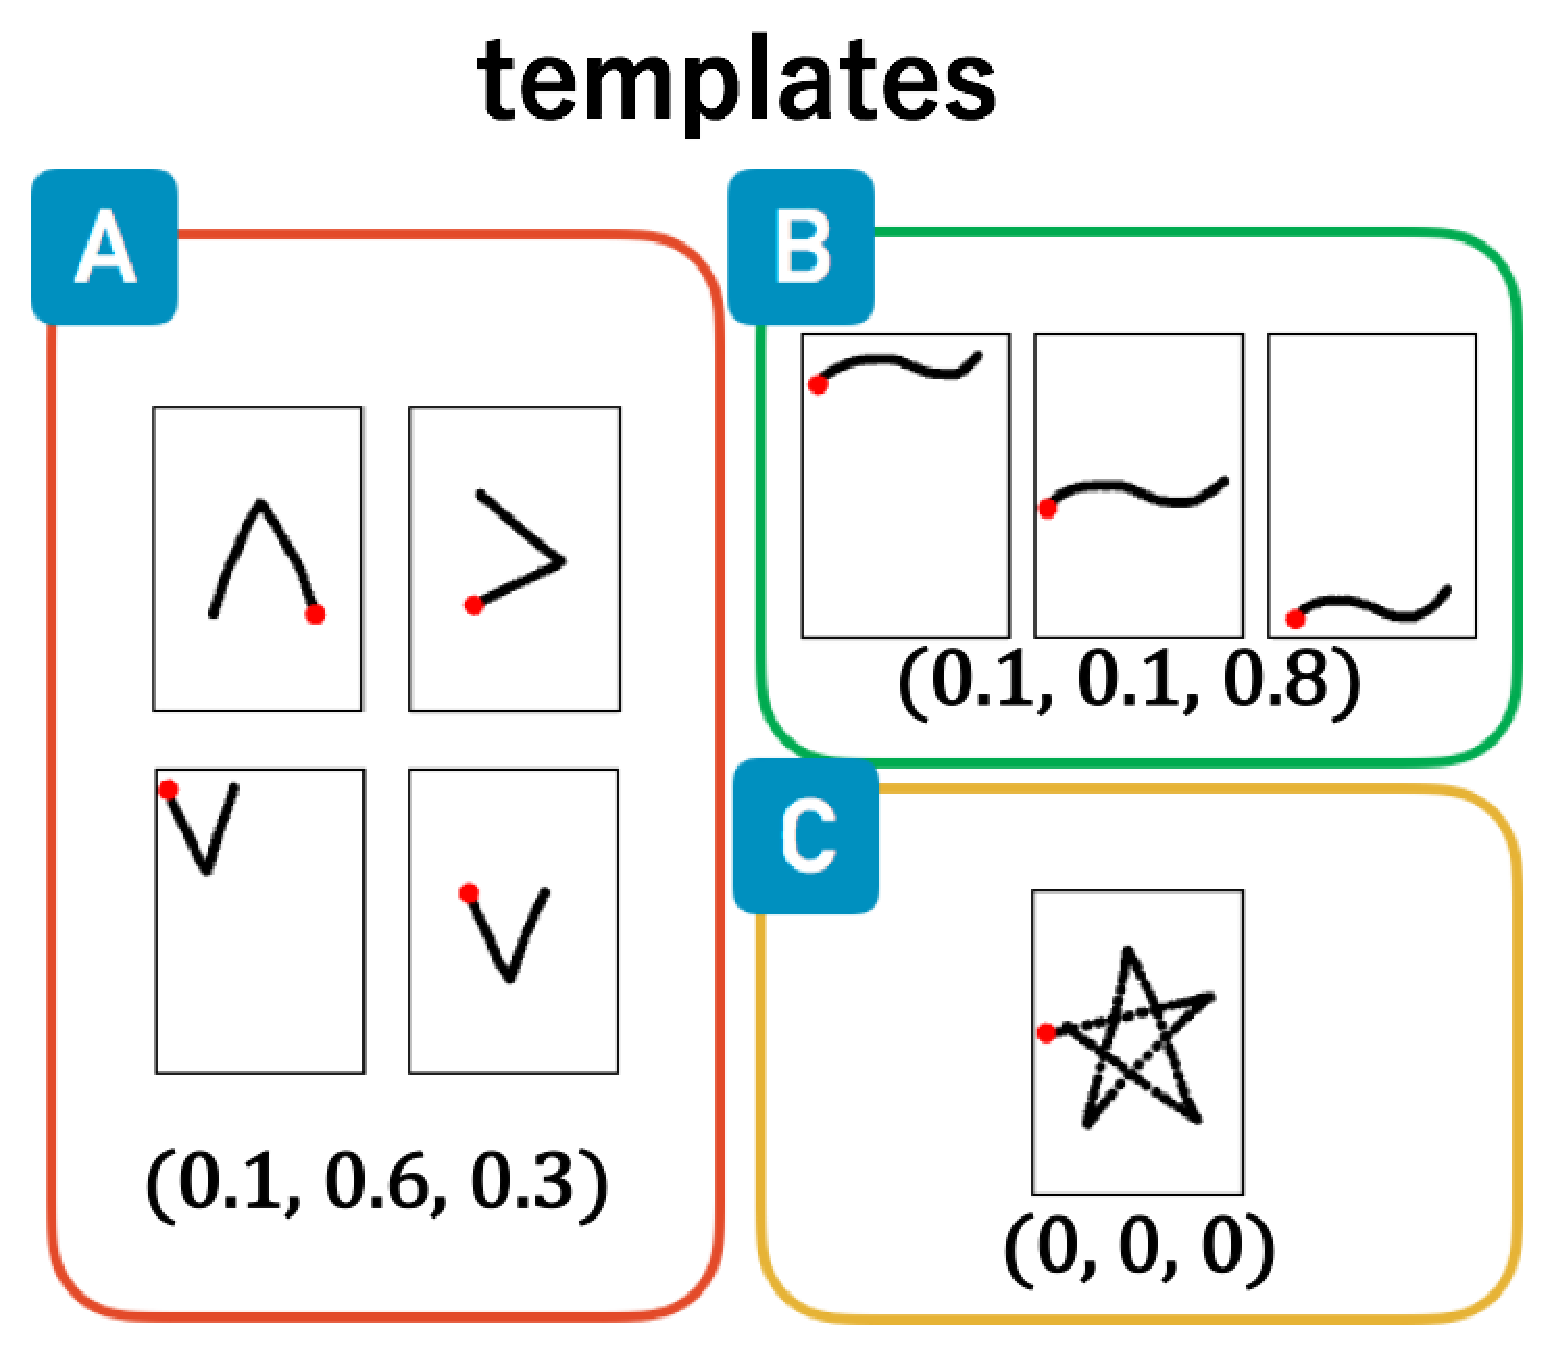
\includegraphics [width=0.7\hsize ]{img/group_weight.eps}
%	\end{center}
%	\caption{Examples of gesture groups and optimal weight values ($Ws$, $Wo$, $Wp$) for each group.}
%	\label{fig:group_weight}
%\end{figure}

\section{ストロークの類似度の定義}

\subsection{大きさ}
\begin{equation}
S{\scriptsize s} = \left \{
\begin{array}{l}
\frac{S'}{S} (S>S') \\\\
\frac{S}{S'} (S'>S')
\end{array}
\right.
\end{equation}


\subsection{向き}
\begin{equation}
S{\scriptsize o} = 1 - \frac{|\theta - \sigma|}{\pi}
\end{equation}


\subsection{位置}
\begin{equation}
S{\scriptsize p} = 1 - \frac{\sqrt{(X - x')^2 + (Y - y')^2}}{\sqrt{W\!idt\!h^2 * H\!ei\!ght^2}}
\end{equation}


\section{形状グループの作成}

\section{最適な重み付けのための実験}
\begin{figure} [h!]
	\begin{center}
		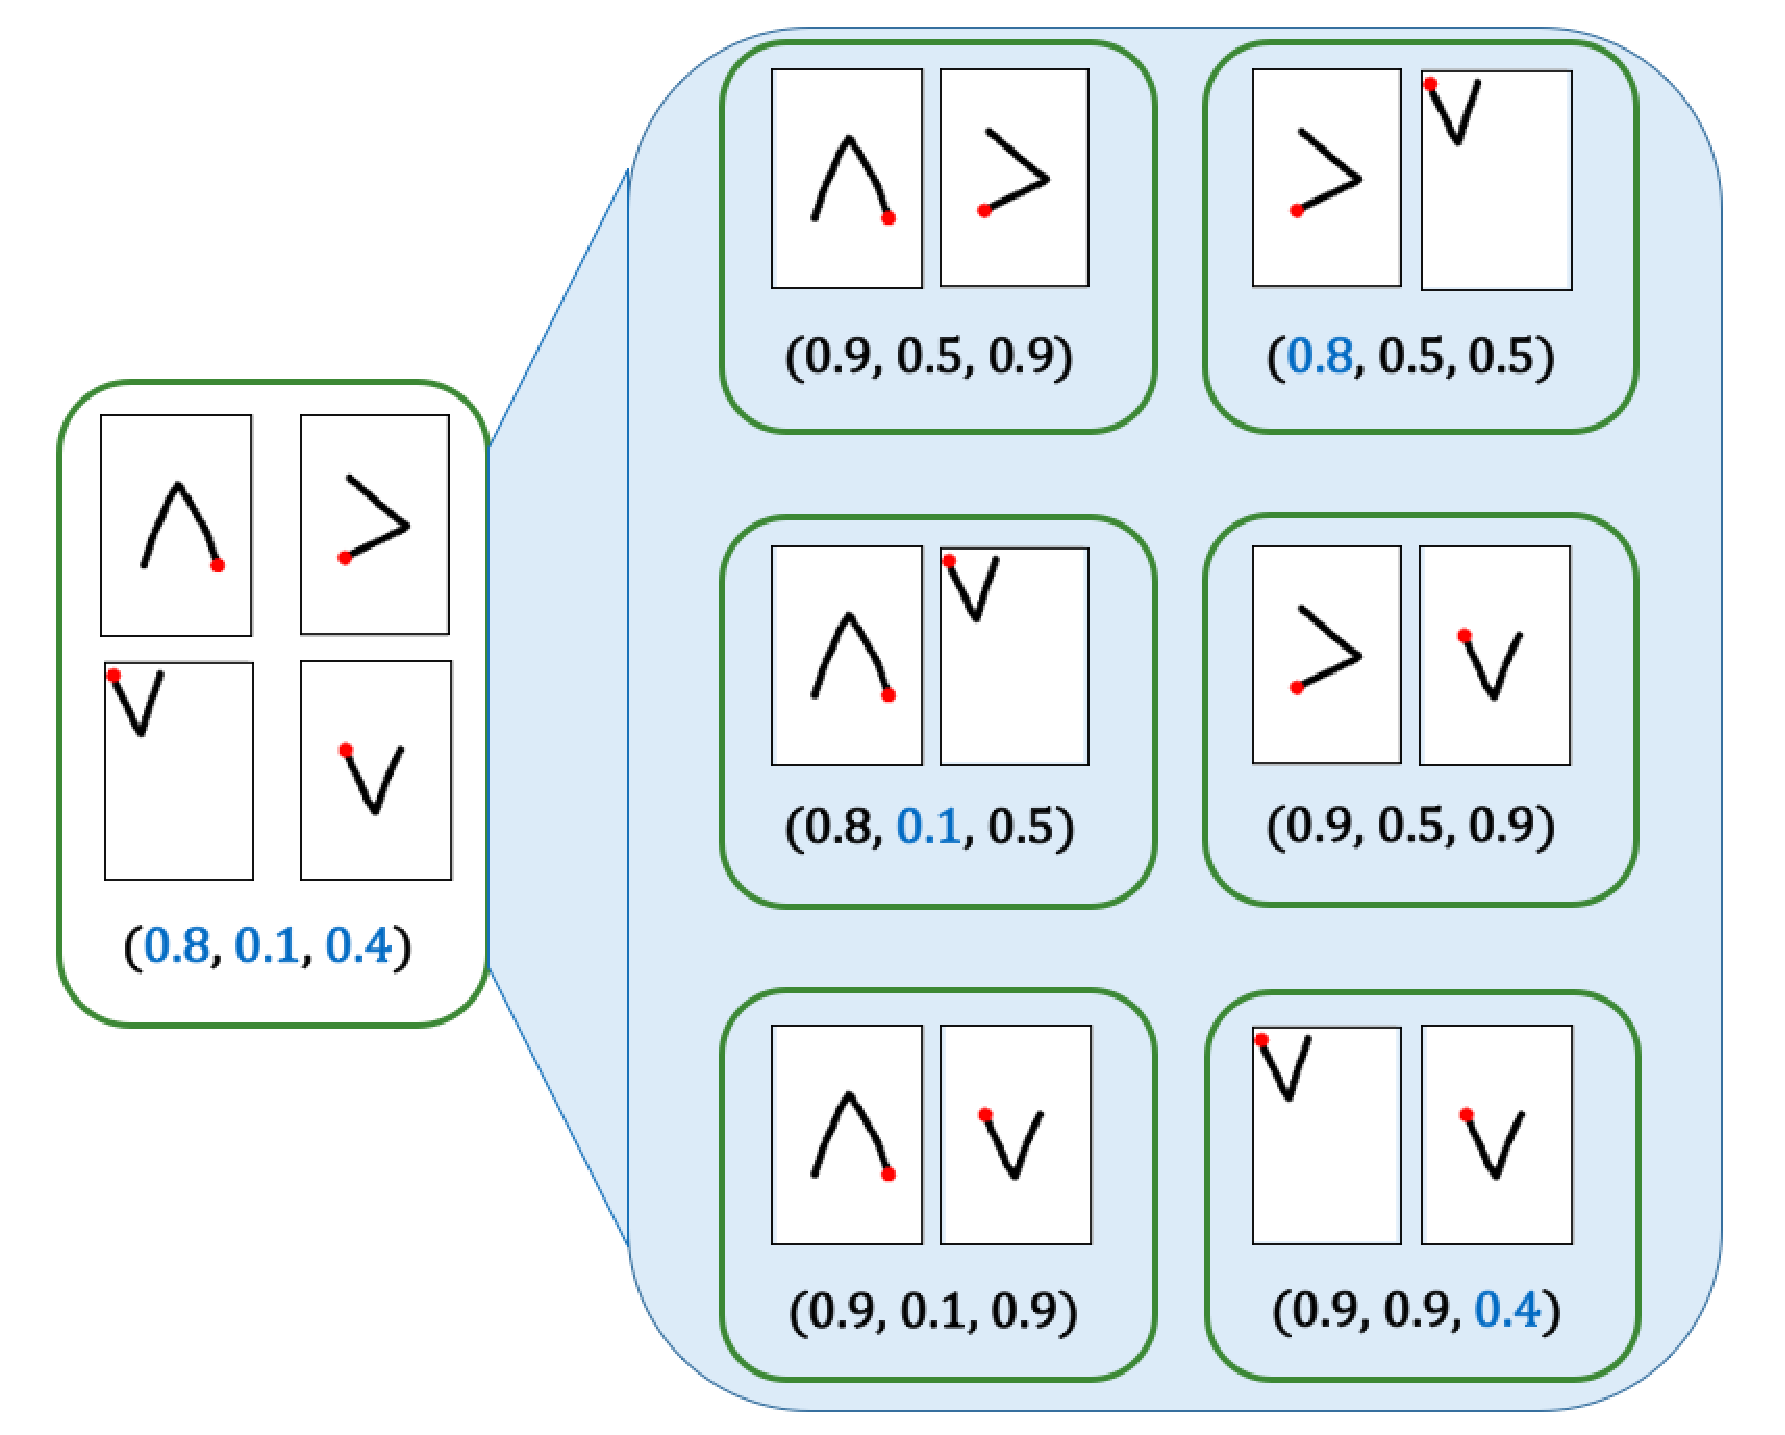
\includegraphics [width=0.8\hsize ]{img/group_similarity.eps}
	\end{center}
	\caption{An Example of how to decide a similarity ($Sts$, $Sto$, $Stp$) of tempaltes in a group gesture, in this case (0.8, 0.1, 0.4) is the similarities.}
	\label{fig:group_similarity}
\end{figure}

\begin{equation}
S{\tiny f} = S{\scriptsize cs} \times W{\scriptsize s} + S{\scriptsize co} \times W{\scriptsize o} + S{\scriptsize cp} \times W{\scriptsize p}
\end{equation}

\begin{figure} [h!]
	\begin{center}
		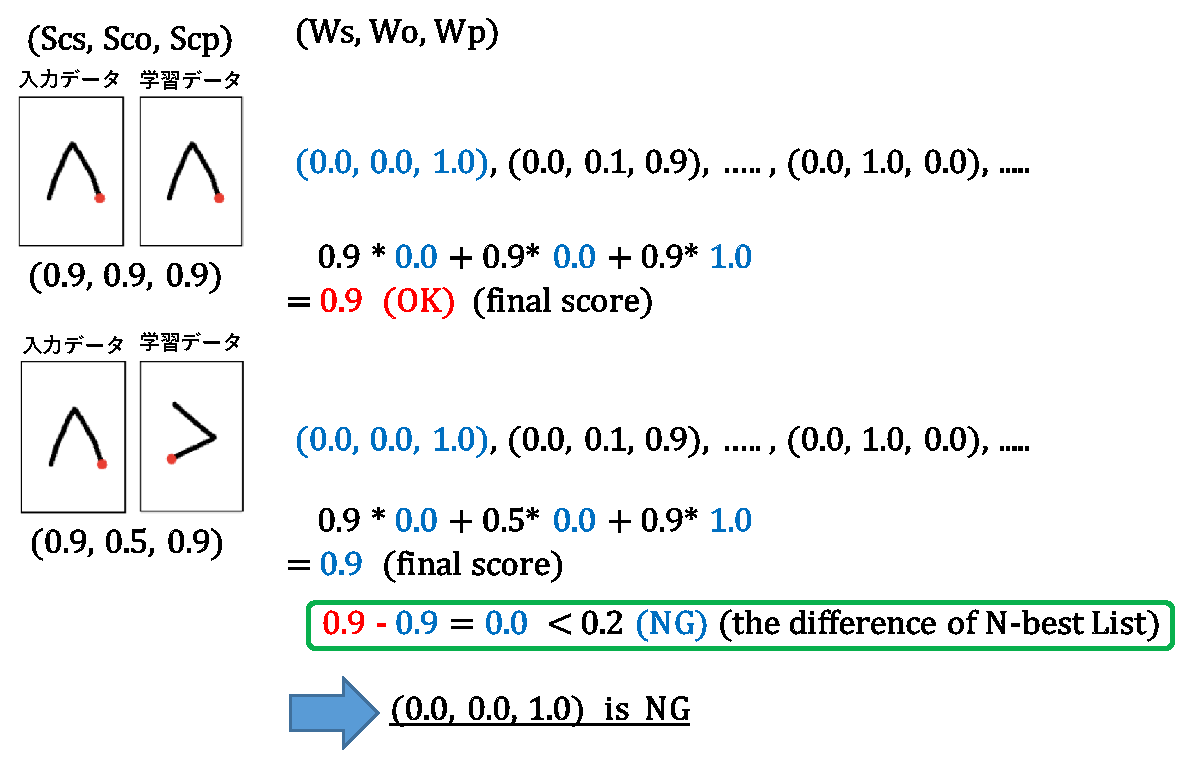
\includegraphics [width=0.8\hsize ]{img/weight_method1.eps}
	\end{center}
	\caption{The procedure to decide the optimal weight values }
	\label{fig:weight_method1}
\end{figure}

\begin{figure} [h!]
	\begin{center}
		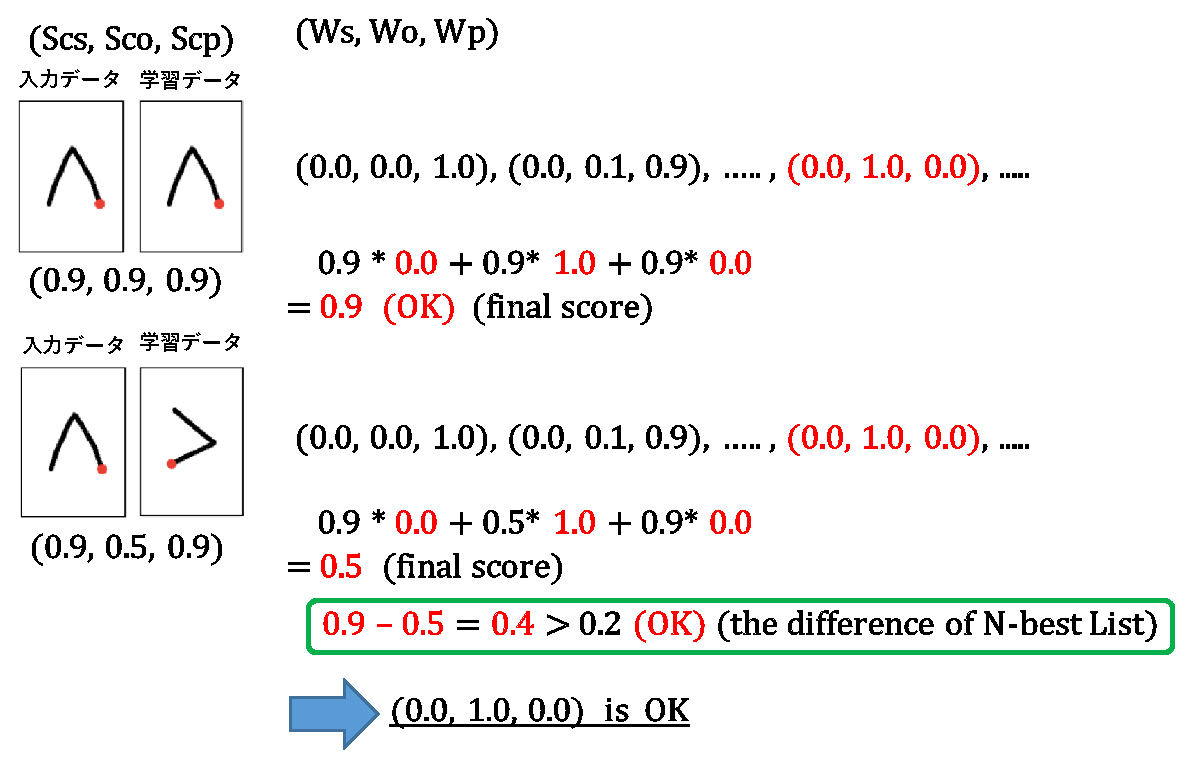
\includegraphics [width=0.8\hsize ]{img/weight_method2.eps}
	\end{center}
	\caption{The procedure to decide non optimal weight values}
	\label{fig:weight_method2}
\end{figure}

\subsection{実験結果}
\begin{figure*} [t]
 \begin{center}
  \includegraphics [width=1.0\columnwidth]{img/weight_graph.eps}
  \caption{The result of the experiment to find the optimal weight values, and blue lines indicates power approximation curves.}
  \label{fig:weight_graph}
 \end{center}
\end{figure*}

\section{ジェスチャの認識}




%評価実験
\chapter{評価実験}
本章にて,重み付けを考慮した\$Vアルゴリズムの性能評価実験を述べる.

\section{実験設計}
\$Vの認識率,認識速度,類似度のN-best Listの1番目と2番目のスコアの差,ジェスチャが一致した時の類似度,ジェスチャが一致した時の類似度の最小値を測定することによってアルゴリズムの性能を評価した.また,認識率,認識速度に関しては,\$Vの拡張元である\$1及び,\$Vと同様に,大きさ,向き,位置に関して異なる手書きジェスチャを識別可能なRubine,DTWと比較した.

実験に用いたジェスチャは,5章と同様,ユーザ調査によって得られたジェスチャを用いる.
また,それぞれの測定方法については,5章において述べた通りに行うが,\$1については,大きさ,向き,位置に関して手書きジェスチャを識別できないため,形状と書き順さえ正しく認識されれば,正しく認識されたとみなした.

\section{実験結果と考察}
\subsection{認識率}
\begin{figure}[!h]
\centering
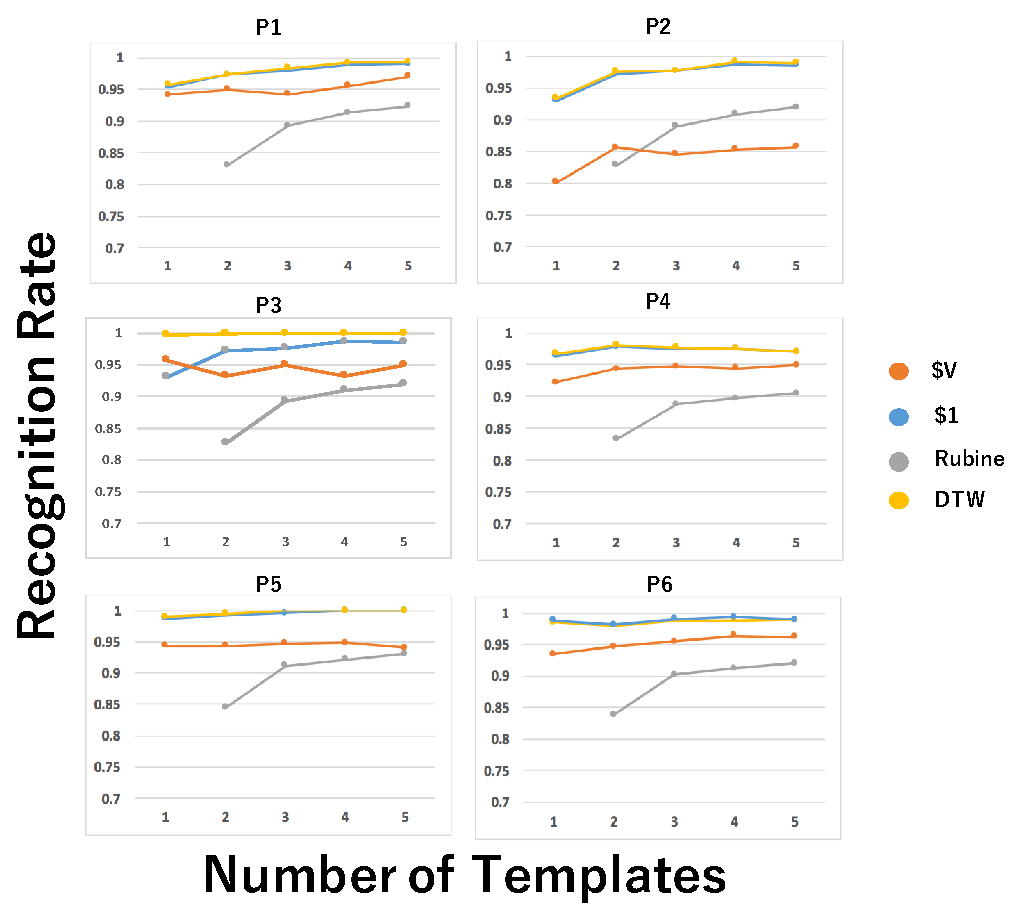
\includegraphics[width=1.0\columnwidth,angle=-90]{img/rec_rate.eps}
\caption{各手法における,被験者ごとの認識率の平均.}
\label{fig:rec_rate}
\end{figure}

図\ref{fig:rec_rate}に各手法ごとの認識率の結果を示す.
それぞれの被験者の平均は,\$Vは93\%~(SD=4.55),\$1は98\%~(1.04),DTWは98\%~(0.86),Rubineは88\%~(2.14)であった.\$Vは\$1とDTWに対し,有意に低かった~(p $<$ 0.01)が,被験者P1,P3,P4,P5,P6に関しては認識率の平均は95\%~(1.27)と高く,\$1と比べて認識率の低下を抑えることができた.\$Vは\$1とは異なり,大きさ,向き,位置に関して異なる手書きジェスチャを識別可能であるにもかかわらず,被験者P1,P3,P4,P5,P6に関しては,認識率はおよそ3\%しか低下しなかった.Rubineと比較した場合は,P1,P3,P4,P5,P6に関しては\$Vは有意に高かった~(p $<$ 0.001).また,重み付けをしない場合と比べても,\$Vは全被験者について認識率は向上し,P6以外は有意に高かった~(p $<$ 0.001).

P2の認識率が低かったのは,P2は別の名前のジェスチャで,形状が酷似したジェスチャが複数存在したため,識別が困難になったことが要因であると考えられる.このように,形状が酷似した手書きジェスチャが別の名前により登録された際に,それらを識別することが困難になることはやむをえないため,アプリケーションユーザにその述べを通知するなどの対処方法が考えられる.また,\$Vは学習データに比例して認識率が高くなるとは言えない.これは,同じジェスチャの学習データを追加するたびに,大きさ,向き,位置それぞれの特徴量を算術平均するため,必ずしも入力データに類似する学習データが存在する可能性が高くなるとは言えないからである.しかしながら,ほとんどの被験者において,少ない学習データにおいて高い認識率を示し,学習データが1つの場合における,全ジェスチャセットの認識率の平均は91.2\%(SD=0.07),学習データが2つの場合は92.2\%(0.04),学習データが3つの場合は92.7\%(0.05),学習データが4つの場合は93.3\%(0.04),学習データが5つの場合は93.2\%(0.05)となった.

\newpage
\subsection{認識速度}
\begin{figure}[!h]
\centering
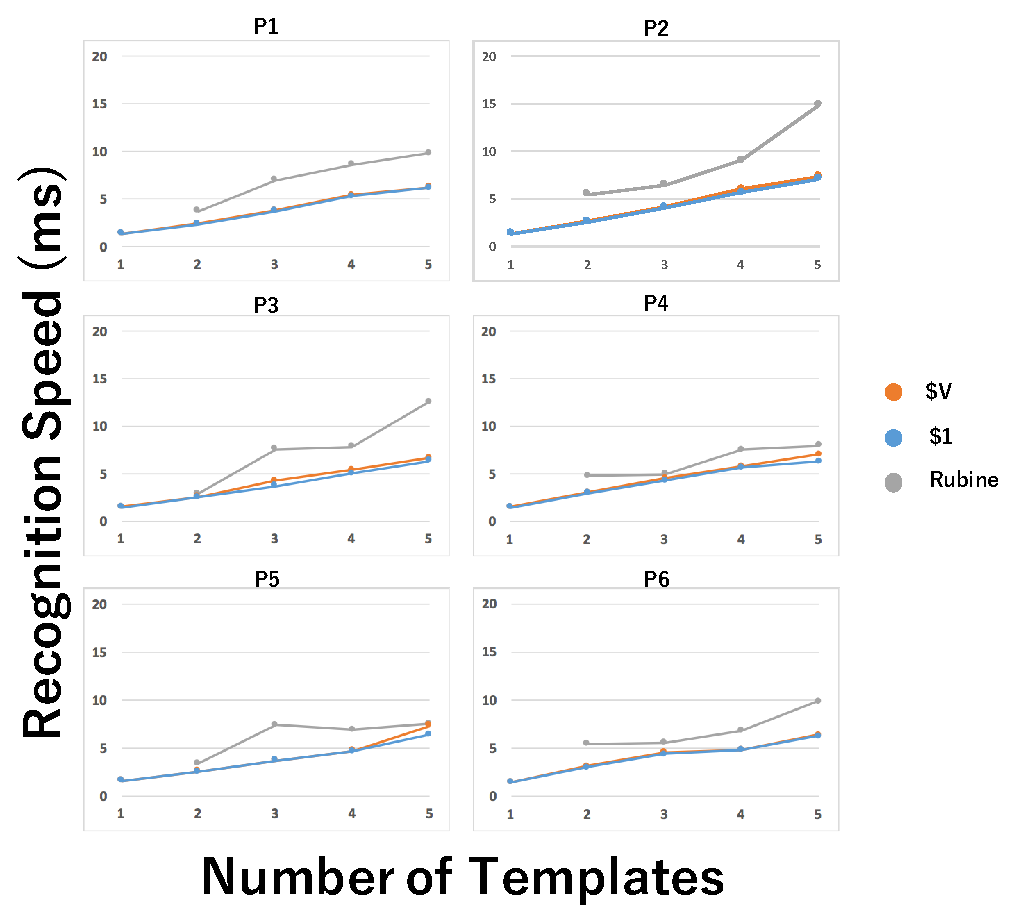
\includegraphics[width=1.0\columnwidth,angle=-90]{img/rec_speed.eps}
\caption{\$V,\$1,Rubineにおける,被験者ごとの認識速度の平均.}
\label{fig:rec_speed}
\end{figure}

\begin{figure}[!h]
\centering
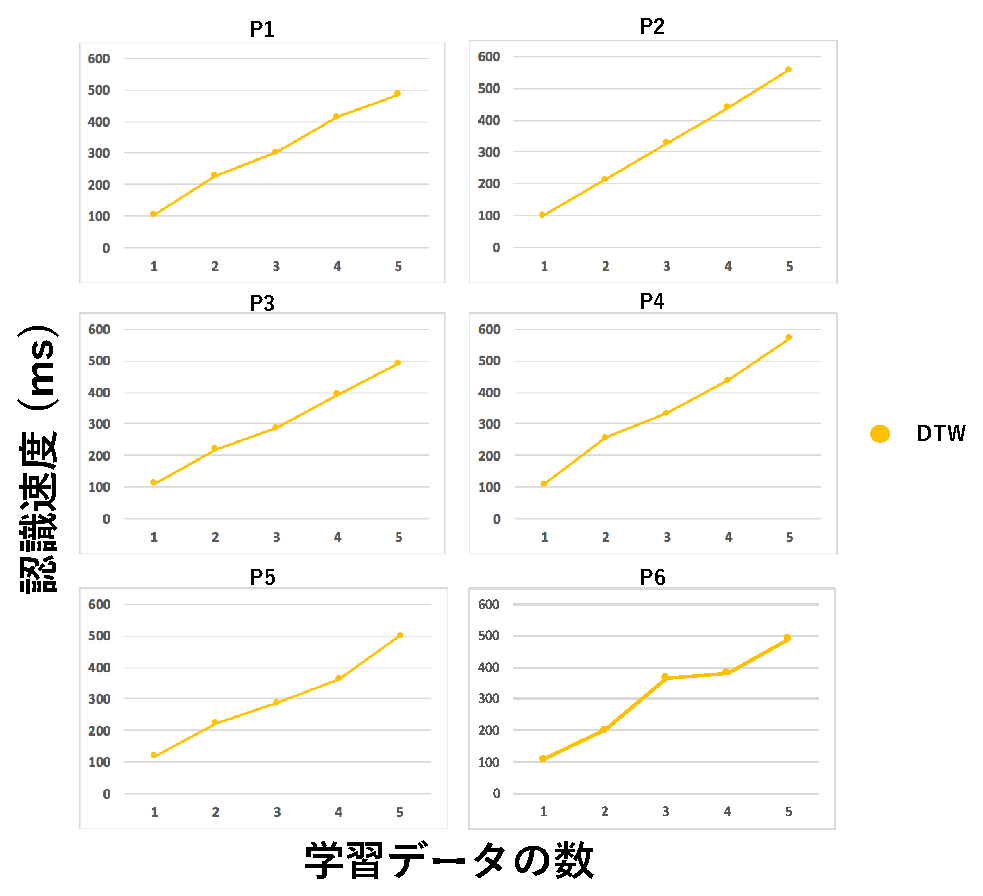
\includegraphics[width=1.0\columnwidth,angle=-90]{img/rec_speed_dtw.eps}
\caption{DTWにおける,被験者ごとの認識速度の平均.}
\label{fig:rec_speed_dtw}
\end{figure}

図\ref{fig:rec_speed}に,\$V,\$1,Rubineの,図\ref{fig:rec_speed_dtw}に,DTWのジェスチャ1つを認識するまでの認識速度の結果を示す.
\$Vの認識速度は,全被験者の平均が,学習データの数が1つの場合~2.6ms (SD=0.2),学習データの数が2つの場合~3.5ms (0.3),学習データの数が3つの場合~4.1ms (0.3),学習データの数が4つの場合~4.9ms (0.3),学習データの数が5つの場合~6.1ms (0.4)だった.また,\$1と認識速度に有意差はなく~(p $<$ 0.001),\$Vは\$1と比べて認識速度の低下を抑えることに成功した.Rubineと比べると有意に速かった~(p $<$ 0.005).DTWの認識速度は図\ref{fig:rec_speed_dtw}に示すように非常に遅く,\$Vの認識速度はDTWのおよそ100分の1であった.また,重み付けをしない場合と比べても,\$Vは全被験者について認識速度は有意差がなかった~(p $<$ 0.001).これは,重み付けのための式を定式化することによって,計算量を削減することに成功したと言える.
また,学習データに比例して認識速度が遅くなることも分かった.

\clearpage
\subsection{識別性能の結果}
\$Vの識別性能の結果を,N-best Listの1番目と2番目のスコアの差及びジェスチャが正しく認識された時の類似度及びジェスチャが正しく認識された時の類似度の最小値を示すことによって述べる.

図\ref{fig:rec_diff}に\$VにおけるN-best Listの1番目と2番目のスコアの差,図\ref{fig:rec_sim}に\$Vにおけるジェスチャが正しく認識された時の類似度,図\ref{fig:rec_min}に\$Vにおけるジェスチャが正しく認識された時の類似度の最小値の結果を示す.
また,図\ref{fig:rec_diff_10}に\$Vにおいて重み付けをしない場合における,N-best Listの1番目と2番目のスコアの差,図\ref{fig:rec_sim_10}に\$Vにおけるジェスチャが正しく認識された時の類似度,図\ref{fig:rec_min_10}に\$Vにおけるジェスチャが正しく認識された時の類似度の最小値の結果を示す.

\$Vにおいて,N-best Listの1番目と2番目のスコアの差について,全ジェスチャセットの平均値はおよそ0.24~(SD = 0.10)となった.また,ジェスチャが正しく認識された時の類似度の平均値は0.94~(SD=0.04)となり非常に高いと言えるが,ジェスチャが正しく認識された時の類似度の最小値は被験者によってばらつきが生じ,平均値はおよそ0.83~(0.14)であった.

N-best Listの1番目と2番目のスコアの差の全ジェスチャセットの平均値は,重み付けをしない場合と比べて有意差はなかった~(p $<$ 0.01)が,P6は有意に高く~(p $<$ 0.01),P4は有意に低かった~(p $<$ 0.01).ジェスチャセットによっては,それぞれの特徴量について尤度を持たせることなく,全く加味するあるいはしないということを明確にした方が類似度の差が明確になる場合があると言える.
ジェスチャが正しく認識された時の類似度の平均値は,重み付けをしない場合と比べて,P1,P5の場合は有意に高かった~(p $<$ 0.01)が,P2,P3,P4,P6に関しては,有意差は無かった.
また,ジェスチャが正しく認識された時の類似度の最小値の平均値は,重み付けをしない場合と比べて有意に低かった~(p $<$ 0.01).これは,ジェスチャグループによっては,適した重み付けがされていない場合があり,その場合類似度が低くなるからであると考えられる.

以上を踏まえ,%ジェスチャが正しく認識された時の類似度の平均値が高いことから,
ジェスチャを識別するにあたり,
重み付けは多くのジェスチャグループにおいて適用可能でありが,重み付けを適用することによって類似度が低下する場合,識別性能が低下する場合もあることがわかった.
しかしながら,認識率の結果を見ると,どのジェスチャグループにおいても重み付けをしない場合と比べて有意に高い~(P6は有意差なし).これは,識別性能自体はジェスチャグループによっては低下する場合もあるが,重み付けにより,識別に必要な特徴量が誤って選ばれる可能性が低くなったことが要因であると言える.例えば,特徴量を認識に用いるか用いないかの2通り~(つまり,重み付けしない場合)によってジェスチャを判別する場合,本来,ある特徴量を考慮すべきジェスチャグループにおいて,その特徴量が全く考慮されない場合ある.この場合,そのジェスチャグループの認識率は低下する.

また,\$Vにおいて,ジェスチャが一致した時の類似度の最小値の平均は0.65以上であり,N-best Listの1番目と2番目のスコアの差の平均値は0.15以上であることから,認識のための類似度の閾値を0.5とすることによって,ジェスチャが一致するか否かを判別することが可能となると言える.
%\subsubsection{N-best Listsの1番目と2番目のスコアの差}
\begin{figure}[!h]
\centering
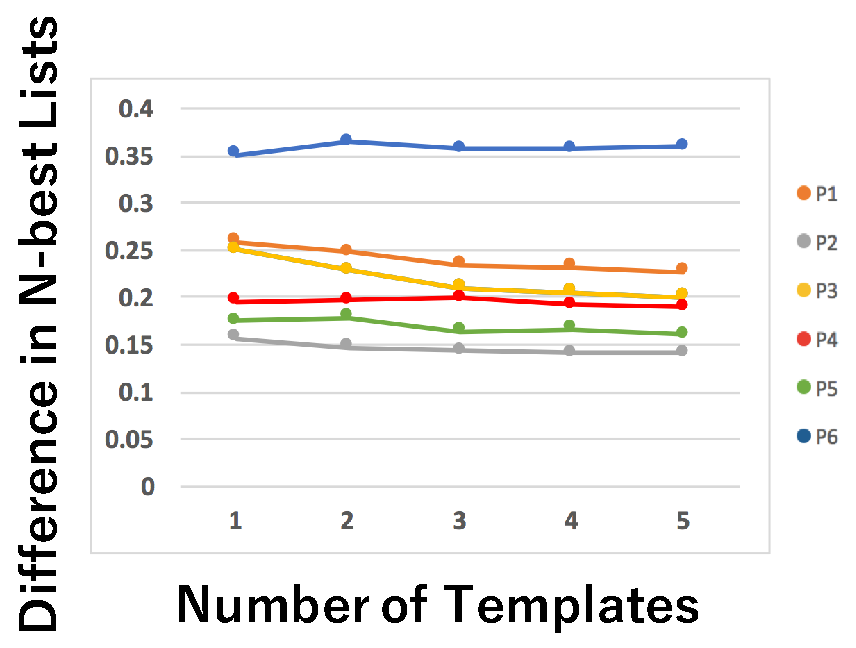
\includegraphics[width=0.7\columnwidth]{img/rec_diff.eps}
\caption{\$Vにおける,N-best Listの1番目と2番目のスコアの差の平均.}
\label{fig:rec_diff}
\end{figure}

%\subsubsection{ジェスチャが正しく認識された時の類似度}
\begin{figure}[!h]
\centering
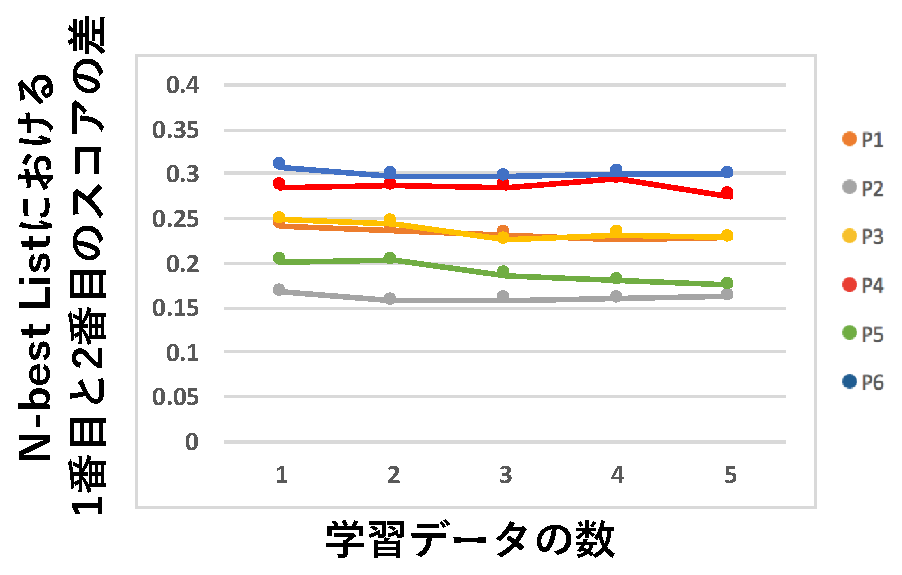
\includegraphics[width=0.7\columnwidth]{img/rec_diff_10.eps}
\caption{\$Vにおいて重み付けをしない場合における,N-best Listの1番目と2番目のスコアの差の平均.}
\label{fig:rec_diff_10}
\end{figure}

%\subsubsection{ジェスチャが正しく認識された時の類似度}
\begin{figure}[!h]
\centering
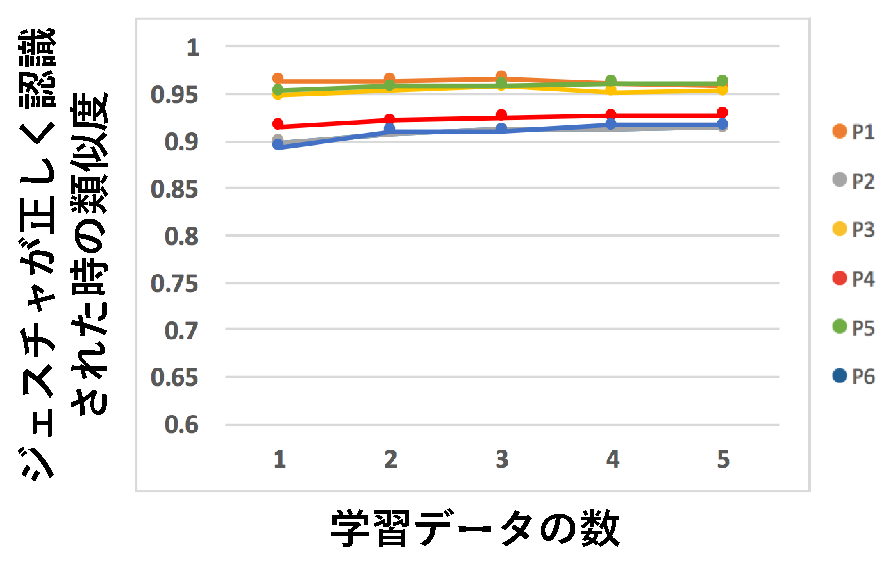
\includegraphics[width=0.7\columnwidth]{img/rec_sim.eps}
\caption{\$Vにおける,ジェスチャが正しく認識された時の類似度の平均.}
\label{fig:rec_sim}
\end{figure}

%\subsubsection{ジェスチャが正しく認識された時の類似度}
\begin{figure}[!h]
\centering
\includegraphics[width=0.7\columnwidth]{img/rec_sim_10.eps}
\caption{\$Vにおいて重み付けをしない場合おける,ジェスチャが正しく認識された時の類似度の平均.}
\label{fig:rec_sim_10}
\end{figure}

%subsubsection{ジェスチャが正しく認識された時の類似度の最小値}
\begin{figure}[!h]
\centering
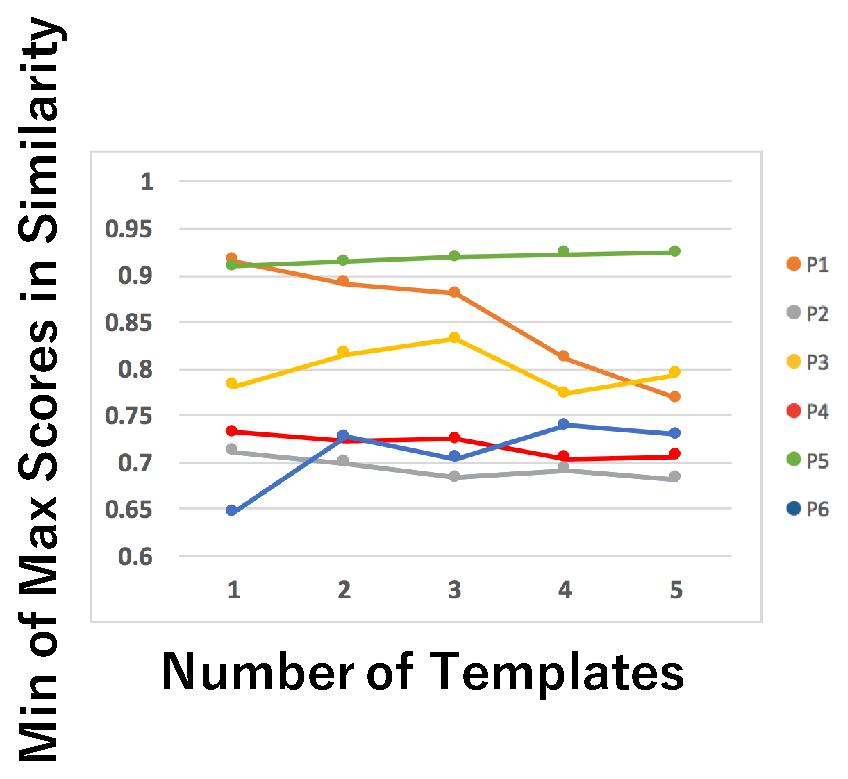
\includegraphics[width=0.7\columnwidth]{img/rec_min.eps}
\caption{\$Vにおける,ジェスチャが正しく認識された時の類似度の最小値の平均.}
\label{fig:rec_min}
\end{figure}

%subsubsection{ジェスチャが正しく認識された時の類似度の最小値}
\begin{figure}[!h]
\centering
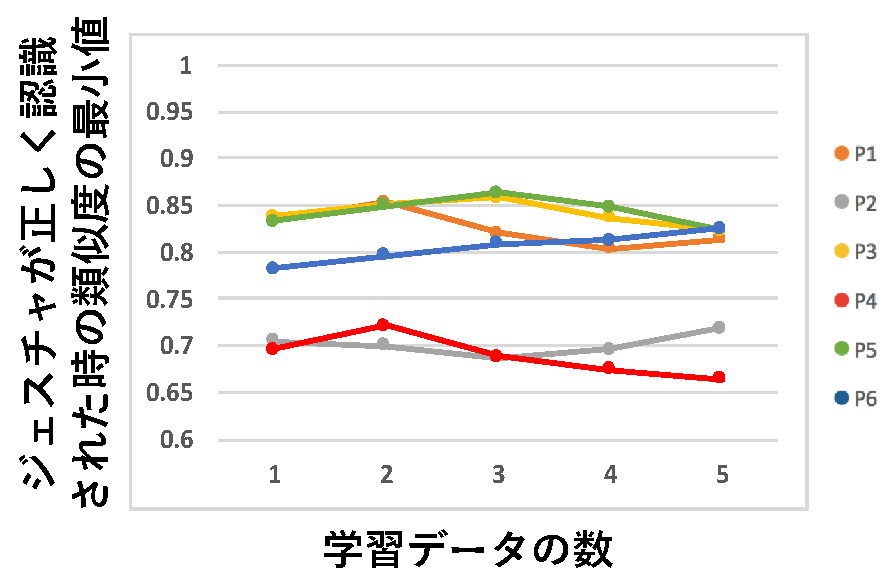
\includegraphics[width=0.7\columnwidth]{img/rec_min_10.eps}
\caption{\$Vにおいて重み付けをしない場合おける,ジェスチャが正しく認識された時の類似度の最小値の平均.}
\label{fig:rec_min_10}
\end{figure}

\clearpage
以上を踏まえ,ジェスチャグループを作成し,ジェスチャグループ内に存在する学習データのみに対し,大きさ,向き,位置の類似度計算をすると認識速度の低下を防ぐことができるという仮説及び,同一ジェスチャグループ内において,他の学習データと類似している特徴量は,認識のための特徴量として用いなければ,認識率の低下を防ぐことができるという仮説は検証され,\$Vは,認識率及び認識速度において高いパフォーマンスを示し,かつ,形状や書き順が同じ手書きジェスチャを大きさ,向き,位置に関して識別可能なアルゴリズムであると言える.

%\TODO{学習データを追加する際の計算量を計測}


%アプリケーション例
\chapter{アプリケーション例}
\$Vを利用したアプリケーション例を本章にて示す.
\$Vは少ない学習データにおいて,高い認識率及び識別性能を示すため,ユーザ定義手書きジェスチャを利用したアプリケーションを開発することができる.
また,同じ形状及び書き順の手書きジェスチャを大きさ,向き,位置に関して識別可能であるため,それらを利用したアプリケーション例を示す.

\section{手書きジェスチャを利用したアプリケーション開発ツールキット}
手書きジェスチャを利用したアプリケーションを開発するためのツールキットを示す.
まず,ユーザは,入力として用いたい手書きジェスチャを実際に手書きジェスチャを入力する端末を用いて学習データとして1つずつ追加していく~(図\ref{fig:flow}a).
すると,\$Vが実装された本ツールキットは,追加された学習データを自動的にジェスチャグループに分類し,それぞれのジェスチャグループごとに,大きさ,向き,位置の特徴量に対する最適な重みを自動計算する~(図\ref{fig:flow}b).
最後に,ユーザは,利用したいアプリケーションにおける処理を実行するAppleScriptあるいはボタンと利用したい手書きジェスチャを対応付けることによって~(図\ref{fig:flow}c),手書きジェスチャを利用したアプリケーションを開発することができる.

\begin{figure} [h!]
	\begin{center}
		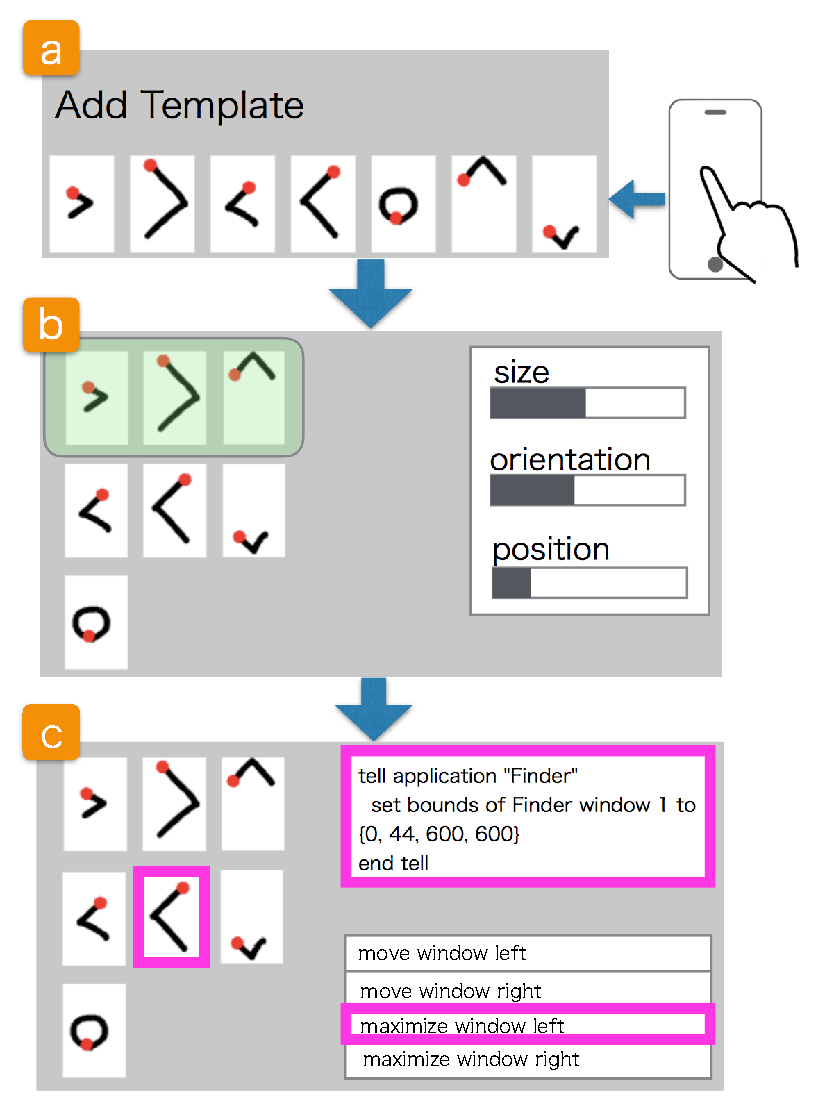
\includegraphics [width=0.7\hsize ]{img/flow.eps}
	\end{center}
	\caption{手書きジェスチャを利用したアプリケーション開発ツールキット.~(a)まず,ユーザはスマートフォンなどの手書きジェスチャを入力する端末を用いて学習データを追加することによって,~(b)\$Vが実装されたツールキットが追加された学習データを自動的にジェスチャグループに分類し,ジェスチャグループごとに重みを計算する.(c)最後にユーザは,アプリケーションにおける処理と手書きジェスチャを対応付ける.}
	\label{fig:flow}
\end{figure}

このツールキット使うことによって,例えば,図\ref{fig:application}のようなメディアプレイヤを開発することができる.
このメディアプレイヤにおいて,再生,巻き戻し,前のメディア,次のメディアなどに対し,同じ書き順及び同じ形状の手書きジェスチャが複数割り当てられており~(図\ref{fig:application}a),それぞれ,大きさ,向き,位置の違いが利用されている.ユーザはスマートフォンを手書きジェスチャの入力端末として用いることによって,PC上のメディアプレイヤを操作することが可能である~(図\ref{fig:application}b).
このようにして,学習データを1つ追加するのみによって,手書きジェスチャを入力として用いるアプリケーションを開発できる.また,大きさ,向き,位置の違いを利用することによって,より実際の動作に即した手書きジェスチャを割り当てることが可能となる.
大きさ,向き,位置の違いを利用できない場合と比べて,利用可能な手書きジェスチャの種類が大きく拡大し,アプリケーションユーザが入力として用いたい手書きジェスチャを考案しやすくなったと言える.

\begin{figure} [h!]
	\begin{center}
		\includegraphics [width=1.0\hsize ]{img/application.eps}
	\end{center}
	\caption{ツールキットを使って開発されたメディアプレイヤの例.~(a)アプリケーションのスクリーンショット,~(b)実際にスマートフォンを用いて入力している場面}
	\label{fig:application}
\end{figure}


%議論
\chapter{議論}
7章までにおいて,\$Vアルゴリズムの詳細及び性能評価を述べた.
本章において,\$Vが今後どのように改善されうるか,あるいは\$Vをどのように発展利用できるかについて議論する.

\section{最適な重み付けの再定義}
5.4節において,認識率及びN-best Listの1番目と2番目のスコアの差を向上させるための重みを実験的に求めた.
しかしながら,ジェスチャグループ内の学習データ間の類似度と重みの関係を示す近似式の決定係数$R^2$は高いとは言えず,今回は,式5.9において示されるように変数を1つにし,段階的に変化させることによって近似式を求めた.
このように決定係数$R^2$が低くなった要因は,ジェスチャグループ内の学習データ間の類似度と重みは,ある程度相関を示したものの,データにばらつきが存在したことであると考えられる.

今回,このデータは,あるジェスチャグループ内の学習データ間の類似度において,ジェスチャが一致した時の類似度の平均値が0.9以上,N-best Listの1番目と2番目のスコアの差が0.2以上となる重みの平均値としてプロットされている.しかしながら,当然ながらこの条件を満たす多くの重みにおいて,具体的な類似度の平均値及びN-best Listの1番目と2番目のスコアの差には違いがある~(例えば,類似度が0.9,N-best Listの1番目と2番目のスコアの差が0.2である重みも存在すれば,類似度が0.99,N-best Listの1番目と2番目のスコアの差が0.4である重みも存在する).このことから,条件を満たす重みを平均するのではなく,高いスコアを示す重みをより重要視することによって,データのばらつきを抑えられる可能性がある.
データのばらつきを抑えることによって,近似式の決定係数$R^2$は高くなり,よりデータを忠実に表す近似式を得られ,認識率の向上あるいは識別能力の向上を実現できるかもしれない.


\section{ユーザに依存しない手書きジェスチャの精度評価}
本研究において,ジェスチャを定義したアプリケーションユーザが,自身が定義したジェスチャを入力した時に,\$Vがどれだけ認識できるかを評価した.今回はアプリケーションユーザが手書きジェスチャ定義する場合を想定しているため,ユーザに依存した手書きジェスチャの評価を行った.しかしながら,アプリケーション開発者が手書きジェスチャを定義する場合,実際に入力するのはアプリケーションユーザであるため,ユーザに依存しない手書きジェスチャにおいても,高い認識率及び高い識別性能が求められる.\$Vは識別に必要のない特徴量の重みを小さくするなどの処理を施すことによって,ロバスト性を極力維持しているため,ユーザに依存しない手書きジェスチャにおいて,
重み付けをしない場合と比べて,高い認識率及び高い識別能力を示す可能性が高い.また,\$1,DTW,Rubineとの比較を含め,ユーザに依存しない手書きジェスチャの精度評価を行うことによって,さらなる改善の余地を発見できるであろう.


\section{書き順に依存しないアルゴリズムの導入}
\$Vは\$1の拡張であり,\$1と同様に形状と書き順を同じジェスチャを認識することができるため,図\ref{fig:different_direction}のような形状が同じであっても書き順の異なるジェスチャは別のジェスチャとして認識される.双方を同じジェスチャとして認識してほしい場合には,それぞれのジェスチャを同じ名前で登録する必要がある.
このようなアプリケーションユーザへの負担を解消すべく,書き順に依存しない,つまり形状さえ同じであれば同じジェスチャとみなすアルゴリズムは\$N~\cite{Anthony:2010:LMR:1839214.1839258}において開発されているため,このアルゴリズムを活用することによって書き順に依存しないアルゴリズムを実現することができる.

\begin{figure} [h!]
	\begin{center}
		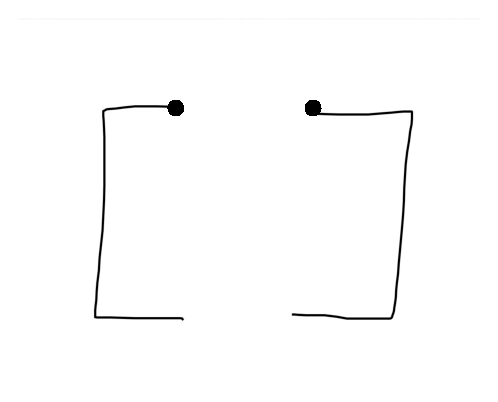
\includegraphics [width=0.5\hsize ]{img/different_direction.eps}
	\end{center}
	\caption{形状が同じであるが書き順の異なる手書きジェスチャの例}
	\label{fig:different_direction}
\end{figure}


\section{スマートフォン以外の端末への応用}
\$Vは,スマートフォンへの手書きジェスチャの入力を想定した,手書きジェスチャ認識アルゴリズムである.
そのため,スマートフォン以外の端末,例えばスマートウォッチやテーブルトップ端末などへの手書きジェスチャの認識アルゴリズムとしても応用できる.
しかしながら,\$1とは違い,大きさ,向き,位置に関して識別可能であるため,それぞれに対する重みを定義する必要がある.
例えば,スマートウォッチはスマートフォンと比べ入力領域が小さいため,大きさや位置の違いを利用しづらく,大きさや位置への重みが小さくなる可能性が高い,反対に,テーブルトップ端末はスマートフォンと比べ入力領域が大きいため,大きさや位置の違いを利用しやすく,大きさや位置への重みが大きくなる可能性が高い.

このように,入力領域を変数として重みを定義することによって,スマートフォン以外の端末への大きさ,向き,位置の違いを利用した手書きジェスチャを認識することが可能になる.

\section{空中手書きジェスチャへの応用}
\$Vは,スマートフォンのような端末への入力を想定しており,認識できる手書きジェスチャは2次元のストロークからなる手書きジェスチャである.これを3次元に応用することによって,Kinectなどの深度センサを用いた~\cite{Tian_kinwrite:handwriting-based}あるいは,端末の加速度を用いた~\cite{Ruiz:2011:UMG:1978942.1978971}ユーザ定義の空中手書きジェスチャを認識することが可能になる.\$3~\cite{Kratz:2010:RSG:1719970.1720051}は\$1を3次元に応用し,空中手書きジェスチャを認識可能にした.このアルゴリズムを活用することによって実現することができる.




%結論
\chapter{結論}
本論文にて,ユーザ定義手書きジェスチャを認識するアルゴリズムである\$Vを開発した.
本論文にてまず,ユーザ調査を行い,アプリケーションユーザは,手書きジェスチャの形状や書き順が同じでも,大きさ,向き,位置の違いを利用したジェスチャを入力したいという要望があることがわかった.これをユーザ定義手書きジェスチャとし,それらを認識するためのアルゴリズムを開発した.
\$Vは\$1を拡張し,\$1のように,アルゴリズムが簡潔である,少ない学習データにおいて高い認識率を示す,認識速度が速い,ロバスト性が高いと行った特徴を持ちながら,\$1とは違い,大きさ,向き,位置に関して識別可能にした.
その際,大きさ,向き,位置に関して不変な\$1と比べて,認識速度及び認識率の低下を抑えるために,ジェスチャグループを作成し,類似度計算するジェスチャの数を減らす,かつ保管されている学習データの類似度をもとに,識別するために必要な特徴量を選定するという手法を用いた.
また,識別するために必要な特徴量を選定する上で,それらの特徴量が識別するためにどれくらい必要であるかを重みによって表現することによって,より尤度の高い認識を可能にした.アプリケーション開発者は,本論文にて示した.学習データ間の類似度と最適な重みの関係式を用いることによって,そのような認識アルゴリズムを容易に実装できる.
評価実験においては,93\%の認識率を示し,N-best Listsの1番目と2番目のスコアの差は0.24であり,高い認識率,識別性能を示した.また,認識速度は\$1と有意差がなく高速であることを示した.また,大きさ,向き,位置が識別可能な既存アルゴリズムと比較し,認識率及び認識速度において高いパフォーマンスを示した.
\$Vアルゴリズムが簡潔であるため,ジェスチャ認識アルゴリズムのライブラリが提供されていない開発環境においても実装可能であるだけでなく,特に手書きジェスチャ認識への深い知識を持たないアプリケーション開発初学者にも,自身のシステムに容易に組み込むことが可能である.
また,\$Vの手書きジェスチャ認識としての改善点及び応用可能性を示した.



\chapter*{謝辞}
本論文を執筆するにあたり,指導教員である志築文太郎准教授をはじめ,高橋伸准教授,嵯峨智准教授,Simona Vasilache 助教には丁寧なご指導及びご助言をいただきました.特に,志築准教授には日々の研究生活の中で、論文の執筆、研究の進め方について手厚いサポートをしていただきました.また,昨年度まで指導教員であった田中二郎教授には研究への取り組み方や大学生,大学院生としての在り方など多くのご指導いただきました.深く感謝申し上げます.
また,インタラクティブ・プログラミング研究室の皆様,特にWAVE チームの皆様及びNERFチームの皆様には、研究についてのアドバイスのみならず,研究以外の生活でも大変お世話になりました.ここまで充実した研究室生活を過ごすことができたのは皆様のおかげです.感謝いたします.
最後に,6年間大学生活を過ごすにあたって支えてくれた家族や,学生生活を共に過ごしお世話になった友人に深く感謝いたします.

\newpage

\addcontentsline{toc}{chapter}{\numberline{}参考文献}
\renewcommand{\bibname}{参考文献}

%% 参考文献に jbibtex を使う場合
\bibliographystyle{jalpha}
\bibliography{master_thesis}
%% [compile] jbibtex sample; platex sample; platex sample;

\appendix

\begin{algorithm}
  \caption{Euclid’s algorithm}\label{euclid}
  \begin{algorithmic}[1]
    \Procedure{Euclid}{$a,b$}\Comment{The g.c.d. of a and b}
    \State $r\gets a\bmod b$
    \While{$r\not=0$}\Comment{We have the answer if r is 0} \label{marker}
      \State $a\gets b$
      \State $b\gets r$
      \State $r\gets a\bmod b$
    \EndWhile
    \State \textbf{return} $b$\Comment{The gcd is b}
  \EndProcedure
\end{algorithmic}
\end{algorithm}

\begin{algorithm}
  \caption*{RESAMPLE(Points, n)}
  \begin{algorithmic}[1]
  \State $I \gets PATH-LENGTH(points) / (n - 1)$
  \State $D \gets 0$
  \State $newPoints \gets points_\textit{0}$
  
\end{algorithmic}
\end{algorithm}






\chapter{ユーザ調査により得られた手書きジェスチャ}

\begin{figure*} [p]
 \begin{center}
  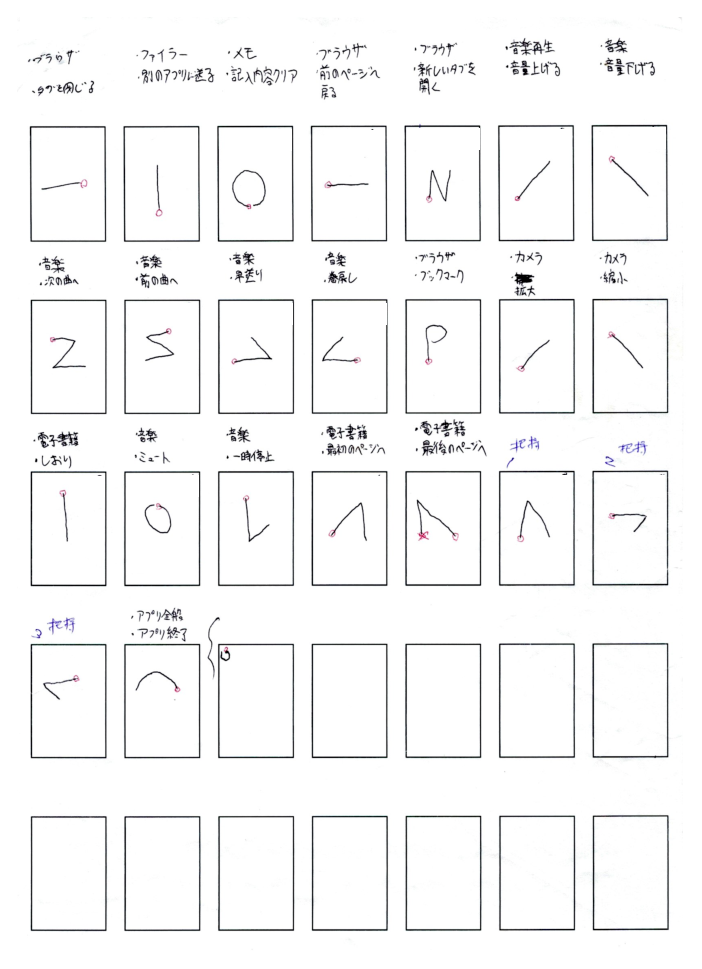
\includegraphics [width=1.0\columnwidth]{img/P1.eps}
  \label{fig:elicitation_example}
 \end{center}
\end{figure*}

\begin{figure*} [p]
 \begin{center}
  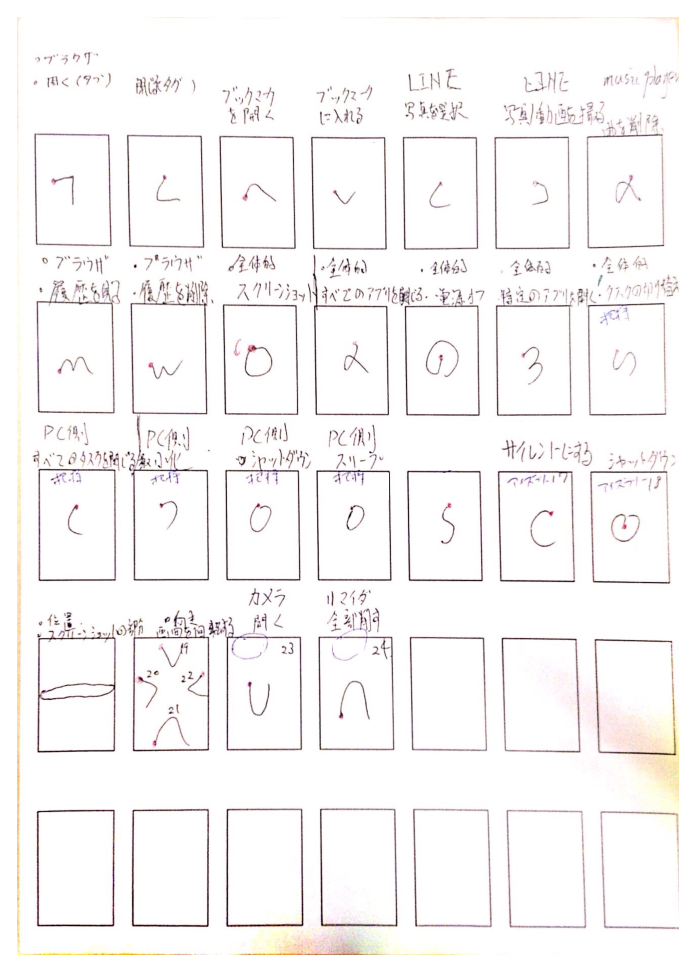
\includegraphics [width=1.0\columnwidth]{img/P2.eps}
  \label{fig:elicitation_example}
 \end{center}
\end{figure*}

\begin{figure*} [p]
 \begin{center}
  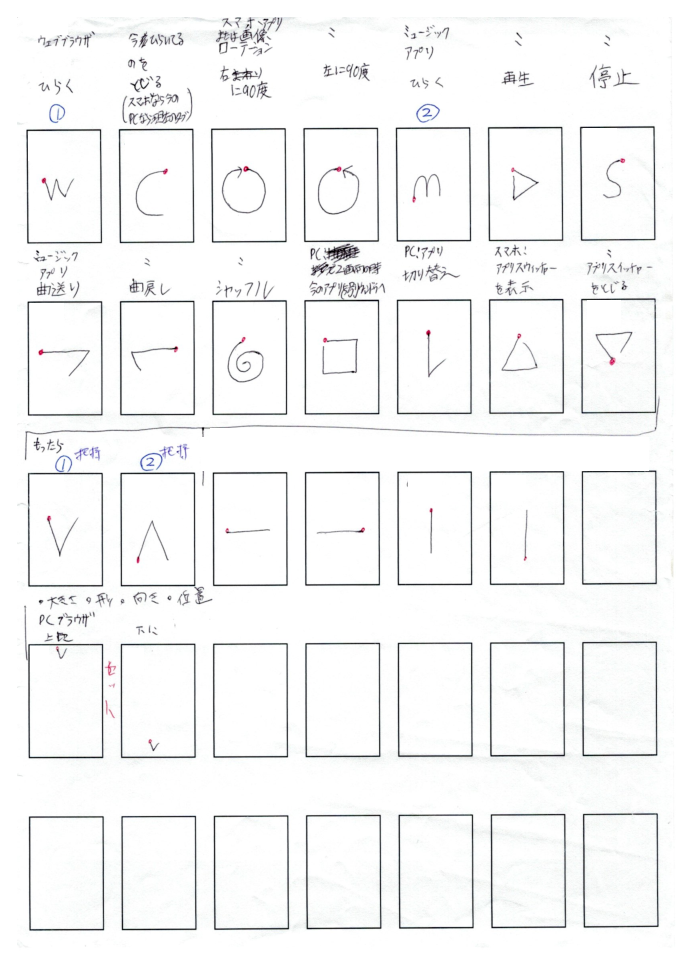
\includegraphics [width=1.0\columnwidth]{img/P3.eps}
  \label{fig:elicitation_example}
 \end{center}
\end{figure*}

\begin{figure*} [p]
 \begin{center}
  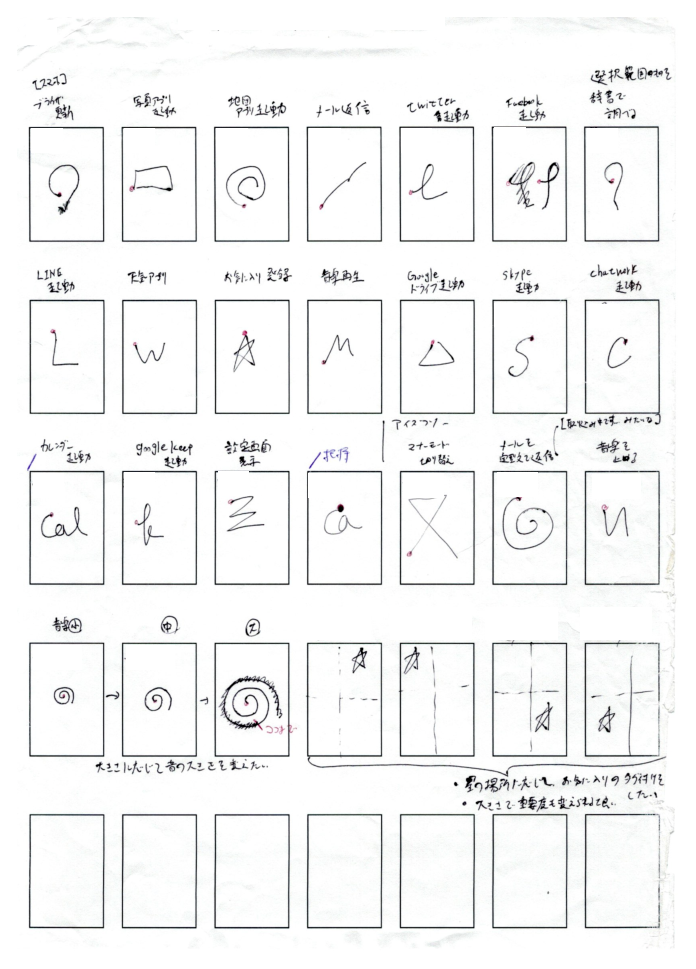
\includegraphics [width=1.0\columnwidth]{img/P4.eps}
  \label{fig:elicitation_example}
 \end{center}
\end{figure*}

\begin{figure*} [p]
 \begin{center}
  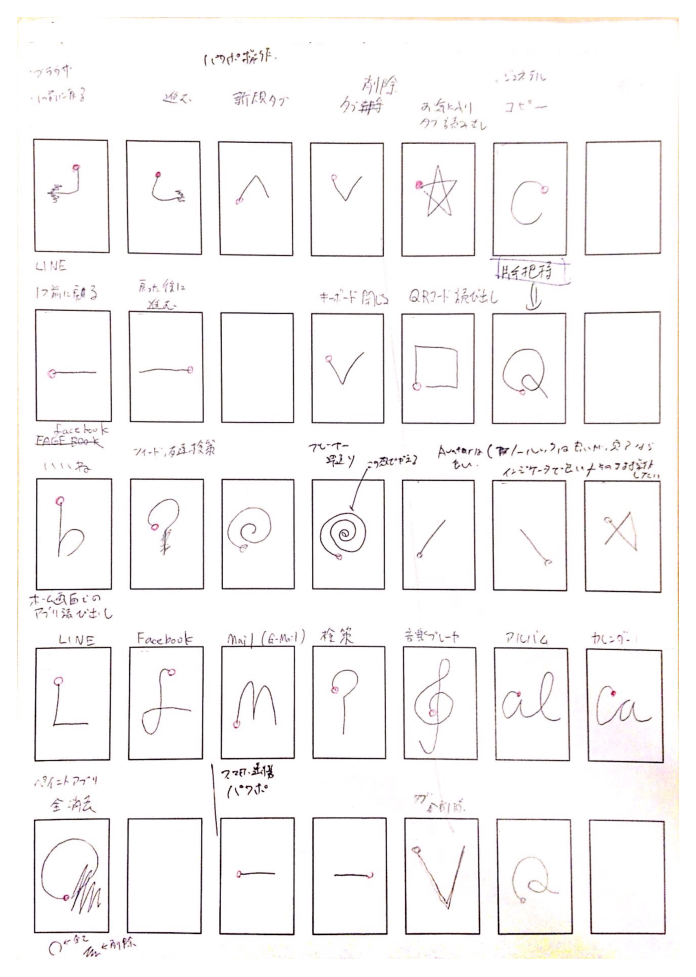
\includegraphics [width=1.0\columnwidth]{img/P5.eps}
  \label{fig:elicitation_example}
 \end{center}
\end{figure*}

\begin{figure*} [p]
 \begin{center}
  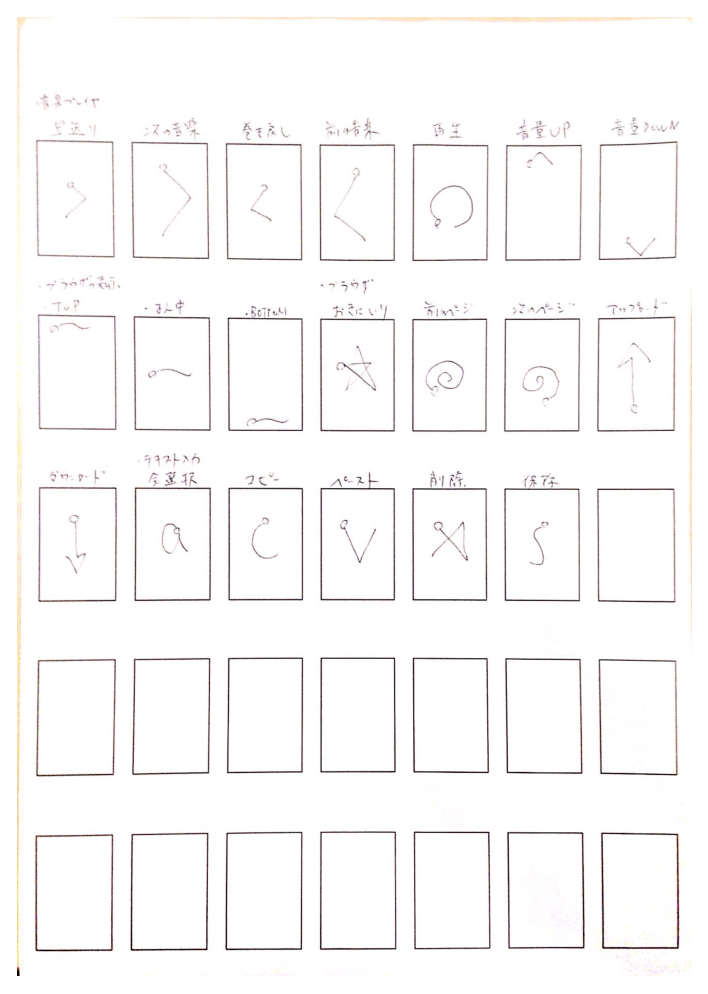
\includegraphics [width=1.0\columnwidth]{img/P6.eps}
  \label{fig:elicitation_example}
 \end{center}
\end{figure*}


\end{document}
